\chapter{Test examples and applications}\label{ch:4-applications}
\markboth{Test examples and applications}{}

In this chapter, we display the performance of the model by tuning it to study the early stages of mouse gastruloid formation. Mouse gastruloids are organoids aggregated from mouse embryonic stem cells (mESCs). The experiments presented in \cite{Oriola_2025} show that:
\begin{itemize}
    \item Cell-cell communication influences cell differentiation and the timing of symmetry breaking in gastruloids
    \item T dynamics is highly dependent on the initial T+ fraction.
\end{itemize}
We implement the model using the feedback expression proposed in the aforementioned study. Our aim is to analyse using the model the effect of cell-cell communication in the differentiation process, showing how spatial organization affects the evolution of stem cells, and to offer a 3D visualization for the early stages of gastruloid formation. A realization of the differentiation process is shown in Figure \ref{fig:aggregate-diff}.

\begin{figure}[h]
    \centering
    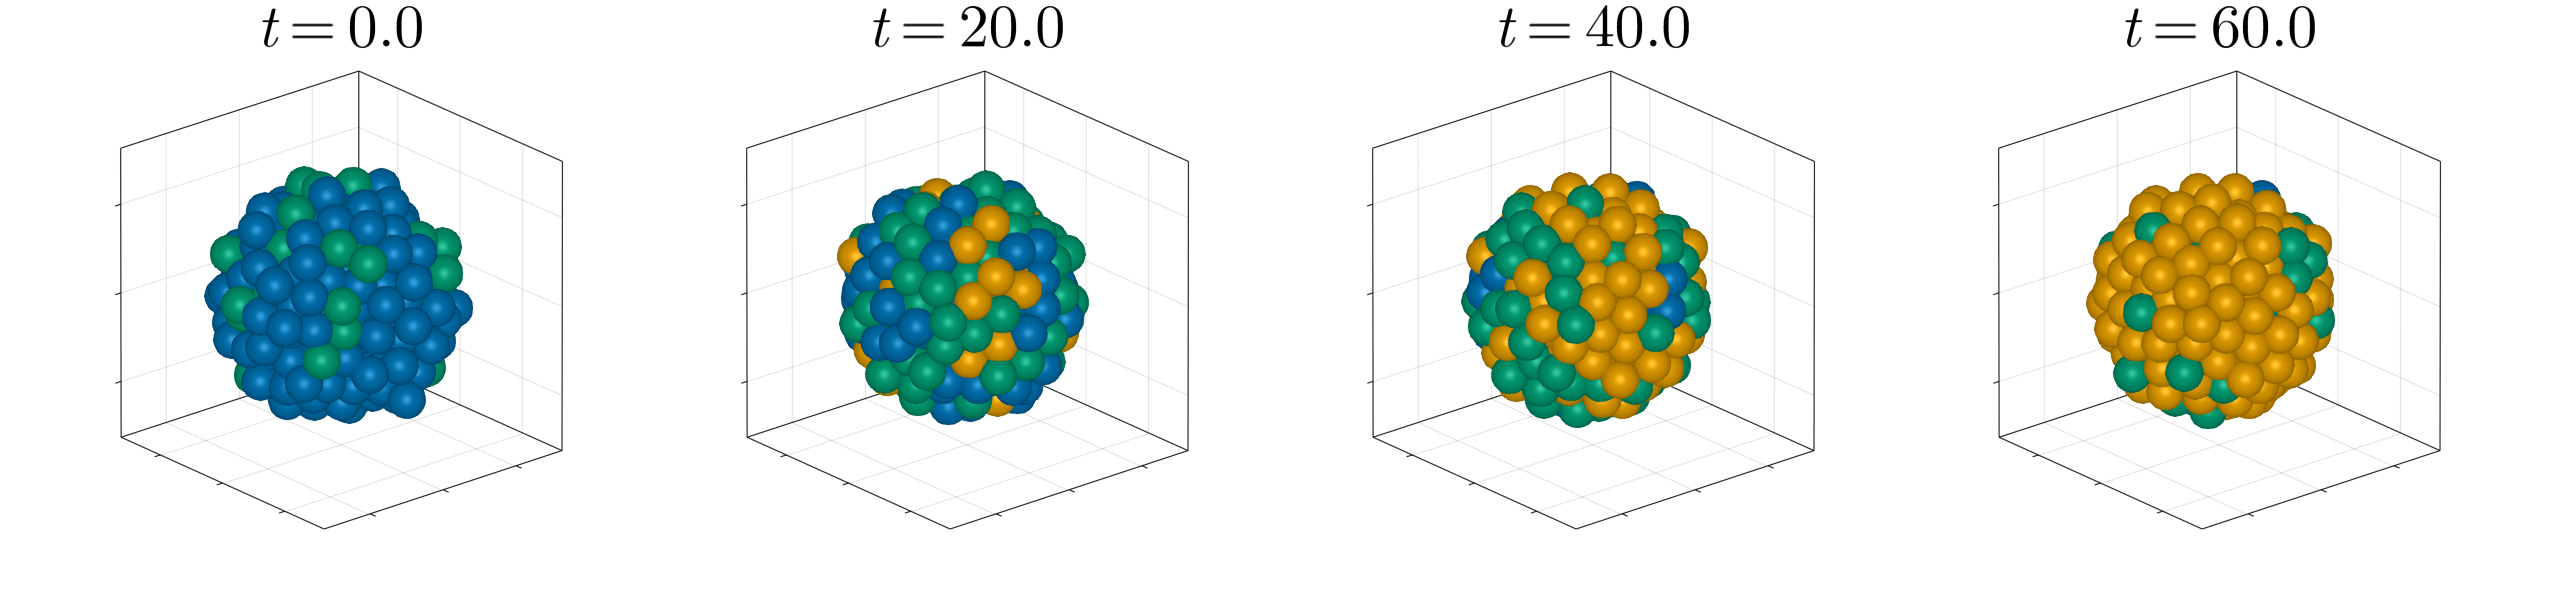
\includegraphics[width=\textwidth]{figures/400/400-aggregate-differentiation.png}
    \caption{Simulation of the differentiation process using cell-cell feedback.\linebreak Time in hours.}
    \label{fig:aggregate-diff}
\end{figure}

First, let us provide a description of the experimental model simulated, along with some insight on the functionality of the simulation.



\section{Physical description}

\subsection{Experimental system}

The simulation is used to recreate the expression of Brachyury (T), a gene that plays an essential role in the formation of embryonic mesoderm. States T- and T+ denote whether the cells express the gene, and are distinguished based on GFP (green fluorescent protein) expression. We do not consider apoptosis (cellular death), as it is not significant in gastruloid formation.

The different stages during early differentiation can be split into three unidirectional states. Let state $A$ represent T-, state $B$ represent T+, and $C$ represent further cellular fates. The experiment consists in creating cell aggregates mixing T+ cells and T- cells under controlled proportions and studying their development. We simulate this by growing an aggregate of cells in state $A$ from a single cell, which resembles the final structure observed in the cultures aggregated experimentally. Then, we initialize a fixed proportion of cells in state $B$ chosen at random. 

The parameters shown in the \hyperref[ch:nomenclature]{Nomenclature} are chosen to mirror the experimental data, taken from the following sources.
\begin{itemize}
    \item Cell radius is taken from \cite{Pillarisetti_2009}.
    \item Average division range is taken from \cite{Roccio_2013}.
    \item Neighbouring and force ranges are taken from \cite{Saiz_2020}.
    \item Differentiation parameters are taken from \cite{Oriola_2025}.
\end{itemize}

Unless stated otherwise, initial aggregates are grown up to $300$ cells, following \cite{Brink_2014}. Next, we compute some measurements to serve as a reference for the rest of the study.


\subsection{Proliferation speed}

In our model, proliferation appears in two contexts: when the initial aggregate is formed and when it occurs during differentiation. In the former, the average division time $\tau_\text{div}$ can be chosen at will as long as the simulation is numerically stable, since the aim is to get the structure. During differentiation, however, the parameter has to be physically accurate in order to tie differentiation dynamics and tissue mechanics. 

In the computation of the initial aggregate, we start from a single cell and grow it up to a given number of cells, whereas in differentiation we start from a system and grow it for a given time. Proliferation requires allocating space before starting the process. Let $N_0$ be the initial number of cells, we expected the number of cells $N_e(t_f)$ after time $t_f$ to increase exponentially,
\begin{equation}\label{eq:growth}
    N_e(t_f) = N_0  2 ^ {\frac{t_f}{\tau_\text{div}}}.
\end{equation}
Due to the stochastic nature of proliferation, the simulation sometimes results in larger values, and so we preallocate $1.4N_e(t_f)$ cells. I Figure \ref{fig:growth} depicts the growth functions for the values of $\tau_\text{div}$ used in each process (see Program \ref{pg:measure-growth}).

\begin{figure}[ht]
    \centering
    \begin{subfigure}{0.4\textwidth}
        \centering
        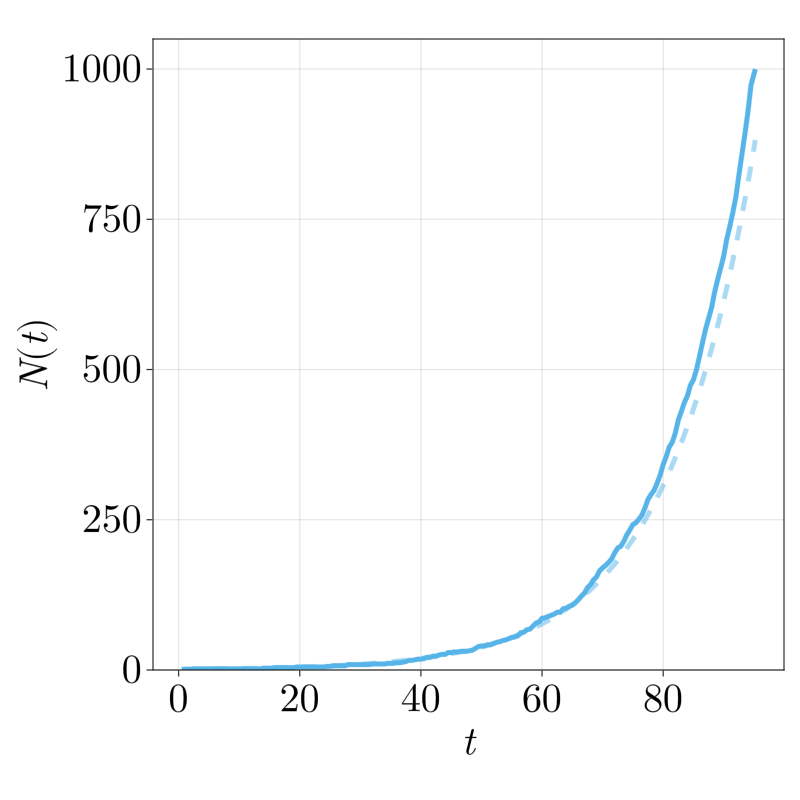
\includegraphics[width=\textwidth]{figures/403/403-growth-prolif.png}
        \caption{Using $\tau_\text{div}=10h$, $N_0=1$, up to $N=1000$.}
    \end{subfigure}
    \hspace{4em}
    \begin{subfigure}{0.4\textwidth}
        \centering
        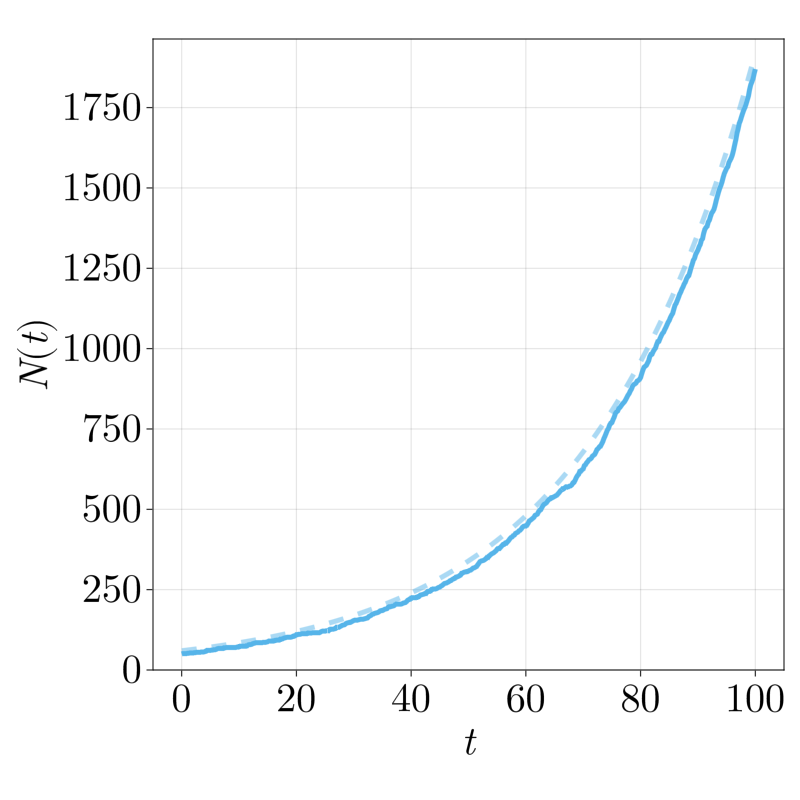
\includegraphics[width=\textwidth]{figures/403/403-growth-diff.png}
        \caption{Using $\tau_\text{div}=20\text{ h}$, $N_0=50$, $t_f=100h$.}
    \end{subfigure}
    \caption{Growth of the aggregate in the simulation.\linebreak Dashed lines correspond to $1.4N_e(t_f)$.}
    \label{fig:growth}
\end{figure}


\subsection{Protrusion force}\label{sec:protrusion-force}

The effect of protrusions is adjusted tuning the following parameters, 
$$\rho=(\tilde D, \tilde k_{p_\text{on}}, \tilde k_{p_\text{off}}).$$
The amount of movement due to protrusions can be adjusted increasing $D$ and $k_{p_\text{on}}$. Greater force strength attracts the cells faster while they are connected, and greater activation rate increases the amount of cells connected to another at each time. In opposition, when protrusions and the growth are disabled, the aggregate tends towards a stable configuration and cells eventually stop moving.

We use the protrusion strength $D$ presented in \cite{Yusko_2014,Moore_2010}. Still, we do not have experimental data for the protrusion activation and deactivation rates. In order to model the random movement of cells seen experimentally using protrusion forces, we set the parameters to
\begin{equation}\label{eq:rho-1}
    \rho_1 = (\tilde D, \tilde k_{p_\text{on}}, \tilde k_{p_\text{off}}) = (10, 20, 10).
\end{equation} 
When the protrusions follow this values, the aggregate slightly contracts, but the number of neighbours remains numerically stable. This happens because cells in the outer layer are connected to cells on the inside.

If we want to increase the amount of cell movement, increasing $\tilde D$ does not suffice: it yields densely packed aggregates as those presented in Section \ref{sec:avg_nbs}. This can be corrected decreasing the protrusion activation rate. We propose the following numerically stable tuple to generate faster cell displacements,
\begin{equation}\label{eq:rho-2}
    \rho_2 = (\tilde D, \tilde k_{p_\text{on}}, \tilde k_{p_\text{off}}) = (50, 2, 0.5).
\end{equation}
Despite the value for the force does not correspond to experimental value, we argue that we can use the tuple as a whole because it causes the sought effect. 



\subsection{Measure of movement}

In this section, we present a method for measuring movement aggregates and apply it to analyse effect of the protrusion force.

When the number of cells $N$ is constant between times $t_0$ and $t_n$, we can use the ensemble average approximation to the mean squared displacement (MSD) to measure the displacement of cells inside the aggregate \parencite{Rosen_2021}. Let $J$ be the number of saved timestamps and $t=\{t_n\}_{n=0,...,J}$ be the associated simulation time.

\begin{definition}
    Let $t_0$ be the initial simulation time. The MSD at time $t_n$ is defined as follows,
    \begin{equation}
        d_2(t_n) = \frac{1}{N}\sum^{N}_{i=1}\left|x_i(t_n)-x_i(t_0)\right|^2.
    \end{equation}
\end{definition}

Let us also define a function to measure the movement in a chosen interval.
\begin{definition}
    The mean square displacement between times $t_1$ and $t_2$  is defined as follows,
    \begin{equation}
        d_2(t_1,t_2) = \frac{1}{N}\sum^{N}_{i=1}\left|x_i(t_2)-x_i(t_1)\right|^2,
    \end{equation}

    and the MSD step at time $t_n, n>0$ as follows,
    \begin{equation}
        g(t_n) = d_2(t_{n-1}, t_n)
    \end{equation}
\end{definition}

Using Program \ref{pg:measure-protrusions}, we carry out measurements for different cases. For reference, cells have a radius of \SI{5}{\pico\meter}, and the maximum distance between cells in 300-cell aggregates is around \SI{65}{\pico\meter}.

When growth stops, cell move towards a stable configuration, and when active forces are neglected ($D=0$), cells gradually stop moving. We plot the first \SI{120}{\hour} of this process and the MSD step at each timestamp in Figure \ref{fig:msd-fp0}.
\begin{figure}[h]
    \centering
    \begin{subfigure}{0.4\textwidth}
        \centering
        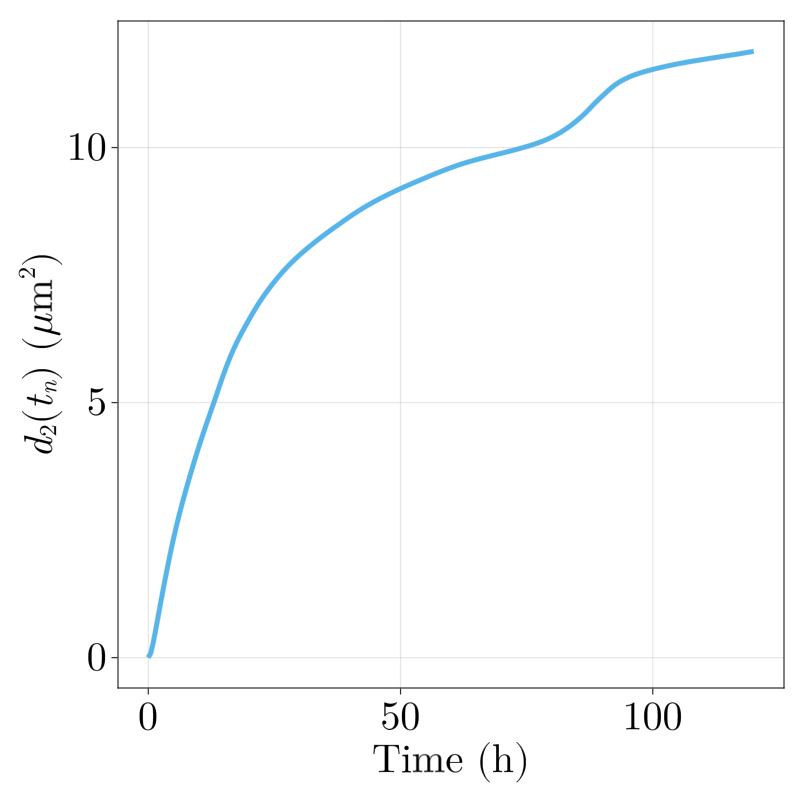
\includegraphics[width=\textwidth]{figures/404/404-mse-fp0-120s.png}
        \caption{MSD.}
    \end{subfigure}
    \hspace{4em}
    \begin{subfigure}{0.4\textwidth}
        \centering
        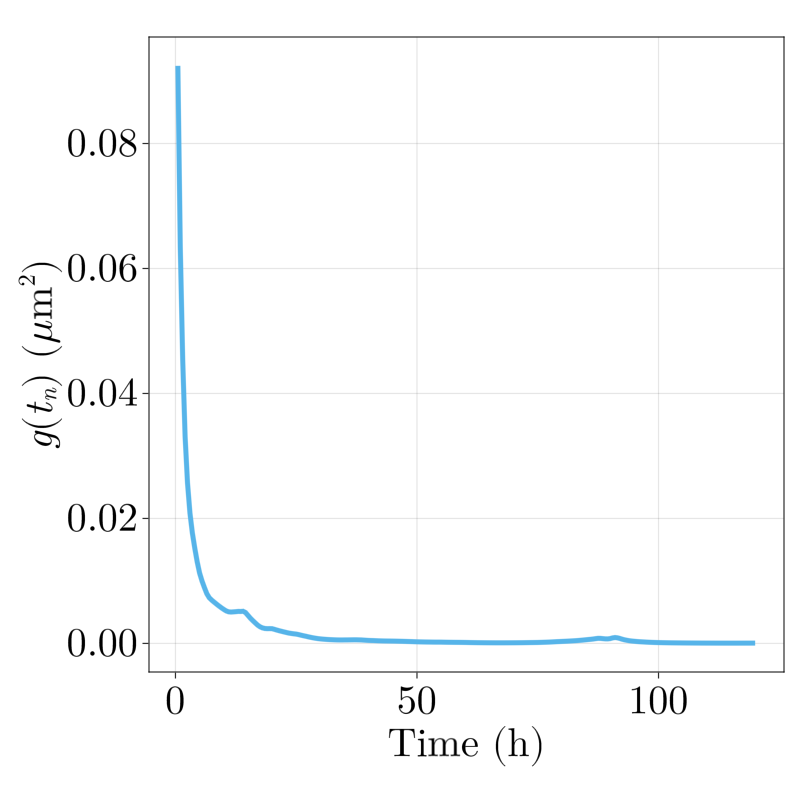
\includegraphics[width=\textwidth]{figures/404/404-step-fp0-120s.png}
        \caption{MSD step.}
    \end{subfigure}
    \caption{Measure of cell movement for $D=0$.}
    \label{fig:msd-fp0}
\end{figure}

We observe that the MSD reaches a plateau at around $t=\text{\SI{60}{\hour}}$. To analyse the effect of protrusions on movement, we initialize aggregates and let them accommodate for this time to obtain more significant data.

Figure \ref{fig:msd-fp50} shows the effect of the protrusion configuration $\rho_2$. The MSD shows linear growth, which indicates diffusive behaviour, as expected. The MSD step shows the oscillations caused by the activation and deactivation of the protrusions, and by the cells moving out of the force range of their pairs. Repeating the computations for $\rho_1$ shows analogous results with smaller values.
\begin{figure}[h]
    \centering
    \begin{subfigure}{0.4\textwidth}
        \centering
        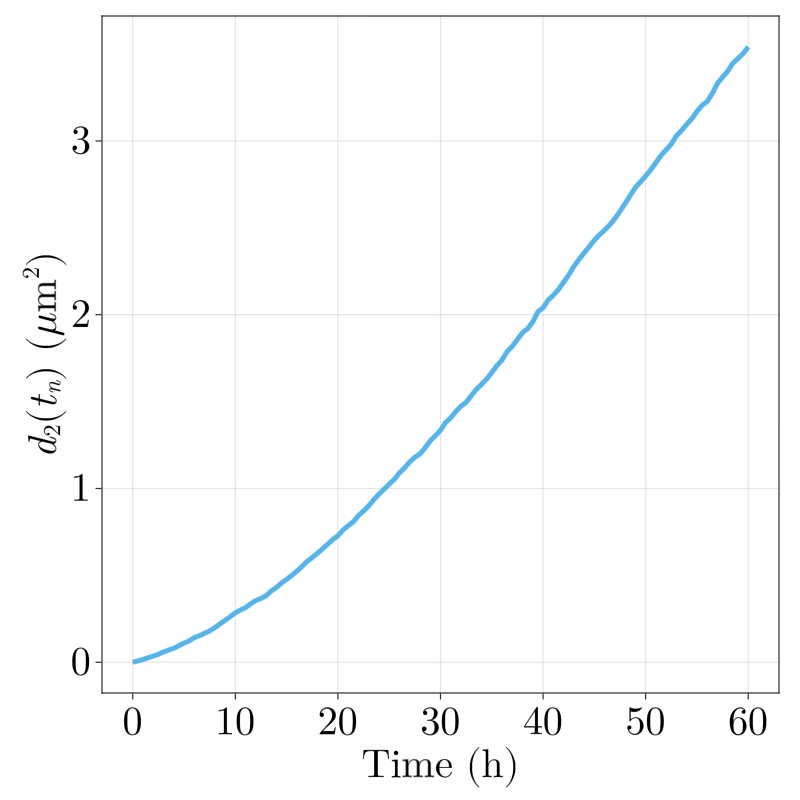
\includegraphics[width=\textwidth]{figures/404/404-mse-fp50.png}
        \caption{MSD.}
    \end{subfigure}
    \hspace{4em}
    \begin{subfigure}{0.4\textwidth}
        \centering
        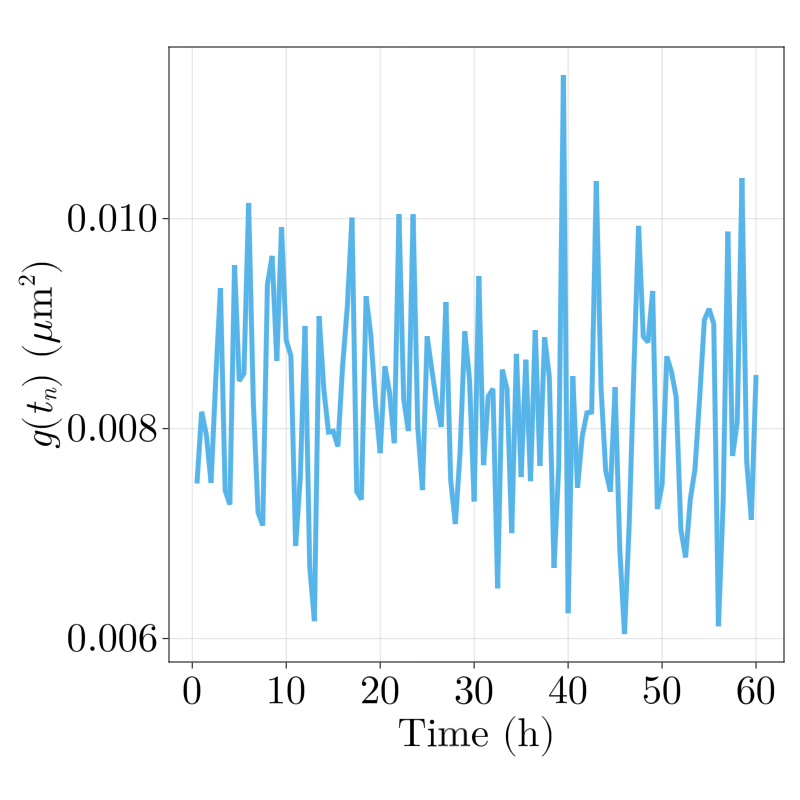
\includegraphics[width=\textwidth]{figures/404/404-mse-step-fp50.png}
        \caption{MSD step.}
    \end{subfigure}
    \caption{Measure of cell movement for $\rho_2$.}
    \label{fig:msd-fp50}
\end{figure}


\subsection{Stable timesteps}

The timesteps used for each type of evolution process are shown in Table \ref{tab:timestep}. Evolution with proliferation is more unstable and requires a lower timestep, so we will disable this option if possible. 

\begin{table}[h]
    \centering
    \begin{tabular}{|m{6.5cm}|m{2cm}|}
        \hline
        \textbf{Process} & \textbf{Timestep} \\
        \hline
        Growth of the initial aggregate & 0.002 \\
        \hline
        Evolution without proliferation, \newline protrusions disabled & 0.002 \\
        \hline
        Evolution with proliferation, \newline protrusions enabled & 0.001 \\
        \hline
        Evolution with proliferation, \newline low protrusion strength & 0.0005 \\
        \hline
        Evolution with proliferation, \newline high protrusion strength & 0.0001 \\
        \hline
    \end{tabular}
    \caption{Timestep values for each evolution process.}
    \label{tab:timestep}
\end{table}




\section{Effect of differentiation kinetics on the evolution of the fate proportions}

The results reproduced here were obtained using Program \ref{pg:proportions}.

Next, we simulate the three expressions for the transition rates presented in Section \ref{sec:diff}, referred to as \textit{constant rates} ($p,q$), \textit{mean field feedback} ($r_{A\rightarrow B},r_{C\rightarrow C}$), and \textit{cell-cell feedback} ($r_{A\rightarrow B}^{(i)},r_{B\rightarrow C}^{(i)}$),
\begin{equation}
    \begin{aligned}
        &r_{A\rightarrow B}=\frac{p}{1+K\phi_A},
        &\quad
        & r_{B\rightarrow C}=\frac{q}{1+K\phi_A}\\
        &r_{A\rightarrow B}^{(i)}=\frac{p}{1+K\langle\mathds{1}_A(i)\rangle},
        &\quad
        &r_{B\rightarrow C}^{(i)}=\frac{q}{1+K\langle\mathds{1}_A(i)\rangle}.
    \end{aligned}
\end{equation}


The behaviour of cells is stochastic and the changes we want to observe may be minor, so the results obtained from a realization are not enough to determine the accuracy of the model; a low number of cells can also affect this precision (see Figure \ref{fig:prop-regu}). Thus, we average several realizations to obtain more significant results.

\begin{figure}[ht]
    \centering
    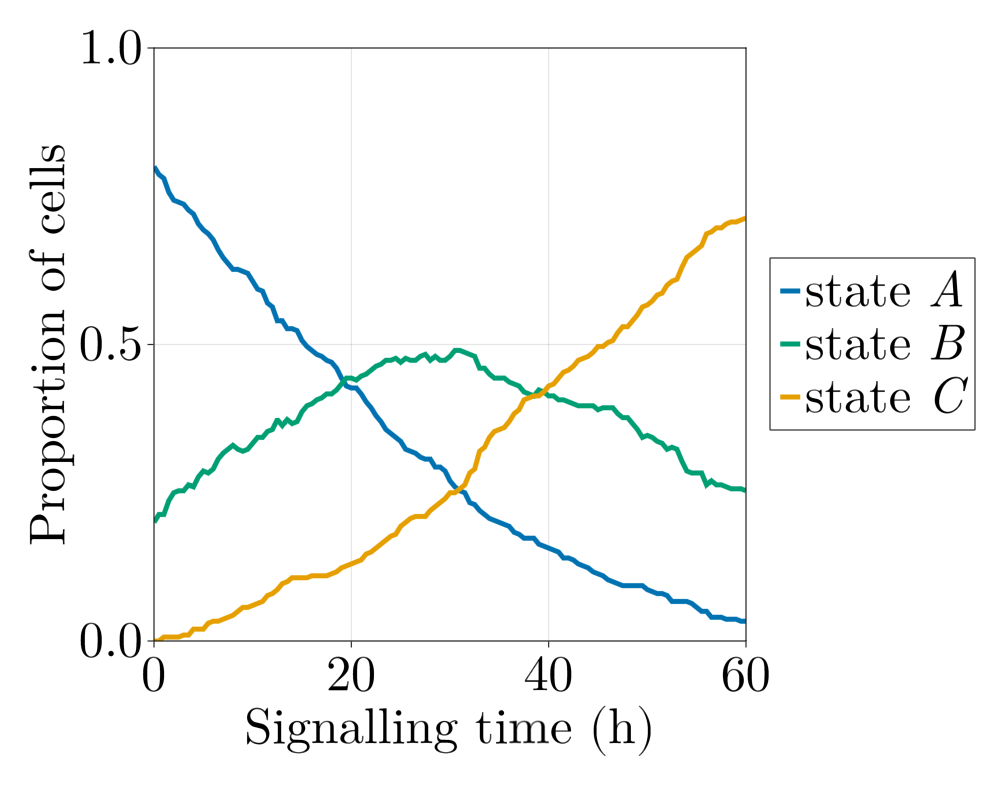
\includegraphics[width=0.47\textwidth]{figures/400/400-proportions-simulation-1ite-fp50-cellcell.png}
    \caption{Proportions over time for a single realization using cell-cell feedback.}
    \label{fig:prop-regu}
\end{figure}


\subsection{Differentiation without proliferation}

We can solve the evolution equations for constant rates and for mean field feedback (see Figure \ref{fig:prop-solutions}). We compute our results for these cases to assert that the differentiation is properly implemented.

\begin{figure}[ht]
    \centering
    \begin{subfigure}{0.47\textwidth}
        \centering
        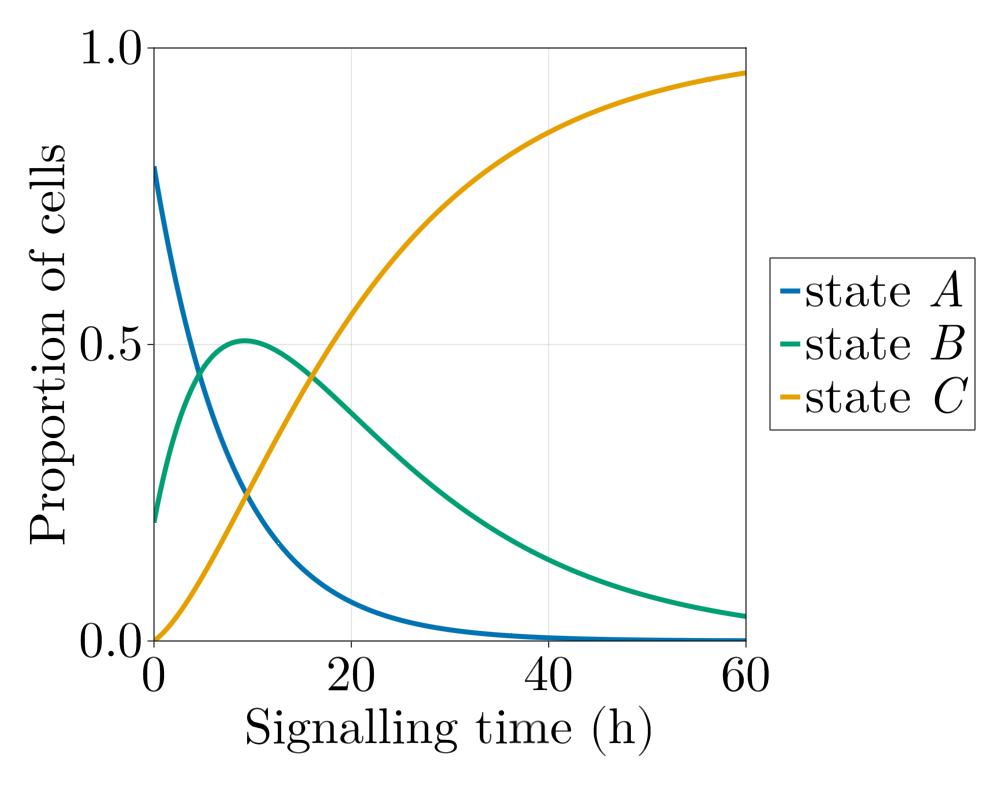
\includegraphics[width=\textwidth]{figures/405/405-proportions-solution-constant.png}
        \caption{Using constant rates.}
    \end{subfigure}
    \hfill
    \begin{subfigure}{0.47\textwidth}
        \centering
        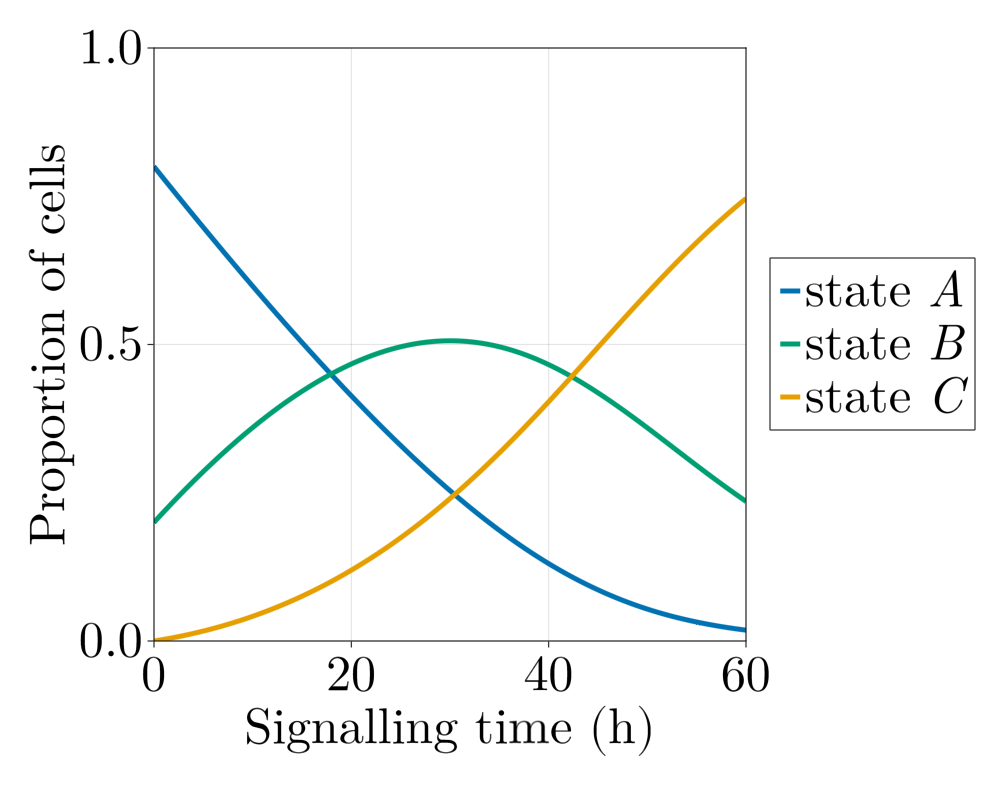
\includegraphics[width=\textwidth]{figures/405/405-proportions-solution-meanfield.png}
        \caption{Using mean field feedback.}
    \end{subfigure}
    \caption{Proportions over time computed using the known solutions.}
    \label{fig:prop-solutions}
\end{figure}

We create an aggregate, stop its growth, and evolve it repeatedly for a time of $t_e=60h$. The initial portion of cells in state $B$ is set to $b=0.2$, and the protrusion is turned off.

The model replicates the behaviour of the solutions using constant rates and mean field feedback, as shown in Figure \ref{fig:prop-itworks}.

\begin{figure}[ht]
    \centering
    \begin{subfigure}{0.47\textwidth}
        \centering
        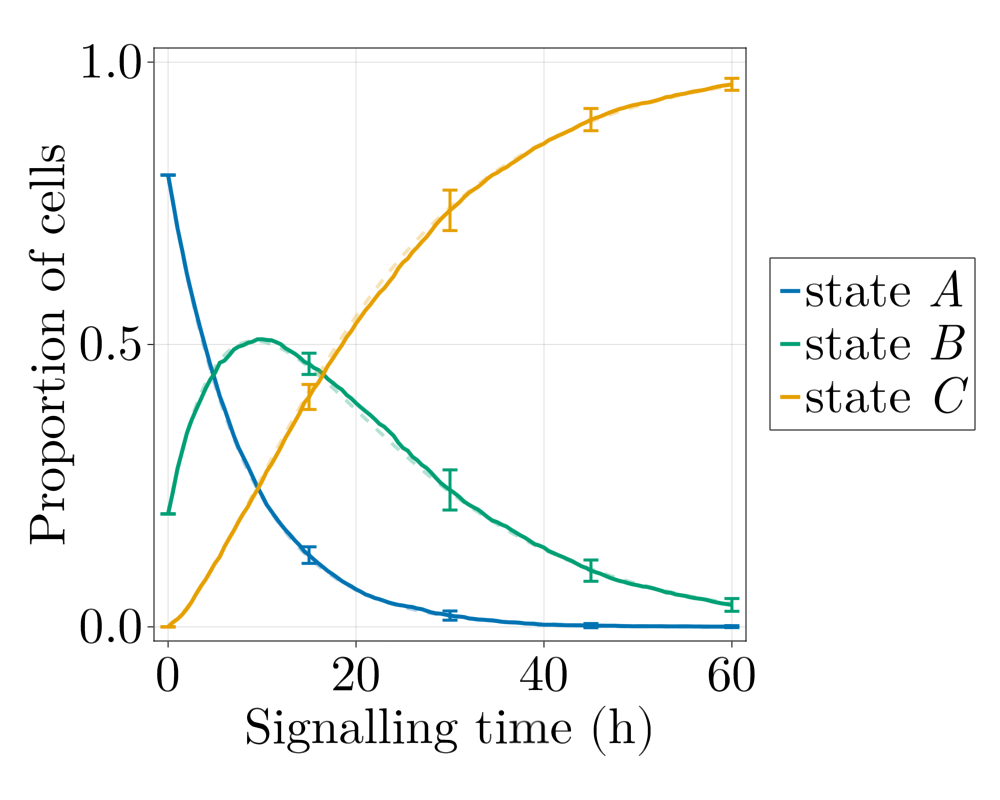
\includegraphics[width=\textwidth]{figures/405/405-proportions-simulation-constant-15ite.png}
        \caption{Using constant rates. Compared to the analytical solution.}
    \end{subfigure}
    \hfill
    \begin{subfigure}{0.47\textwidth}
        \centering
        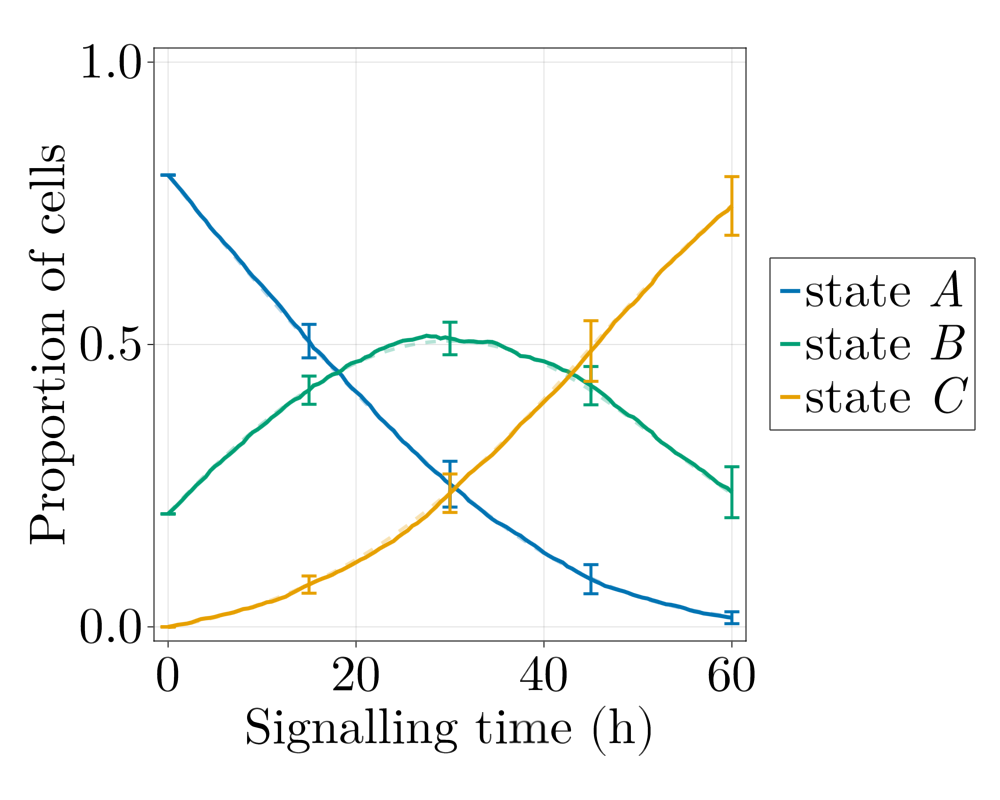
\includegraphics[width=\textwidth]{figures/405/405-proportions-simulation-meanfield-15ite.png}
        \caption{Using mean field feedback. Compared to the numerical solution.}
    \end{subfigure}
    \caption{Proportions over time computed using the simulation. Averaged over 15 realizations. Dashed lines correspond to the solutions in Figure \ref{fig:prop-solutions}, and bars indicate the standard deviation.}
    \label{fig:prop-itworks}
\end{figure}

Once the model is verified, we simulate the nonlinear differentiation kinetics with cell-cell signalling feedback. This effect has only been observed experimentally and the evolution of the proportions cannot be solved analytically, as it accounts for spatial distribution. 

In the first two cases, spatial organization did not affect the differentiation process, so we set $D=0$. However, cell rearrangements might influence the evolution when using cell-cell signalling feedback. We present the results obtained for $D=0$ and $\rho=\rho_1$ in Figure \ref{fig:prop-cellcell}.

\begin{figure}[ht]
    \centering
    \begin{subfigure}{0.47\textwidth}
        \centering
        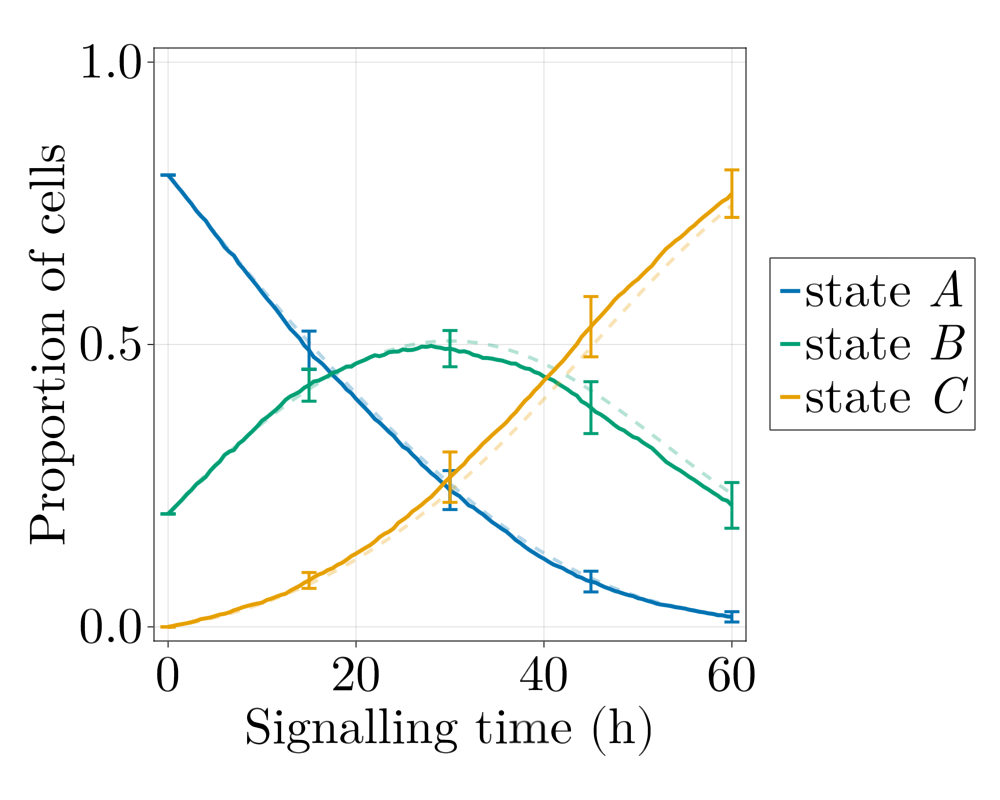
\includegraphics[width=\textwidth]{figures/405/405-proportions-simulation-cellcell-fp0-15ite.png}
        \caption{Turning off protrusions, $D=0$.}
    \end{subfigure}
    \hfill
    \begin{subfigure}{0.47\textwidth}
        \centering
        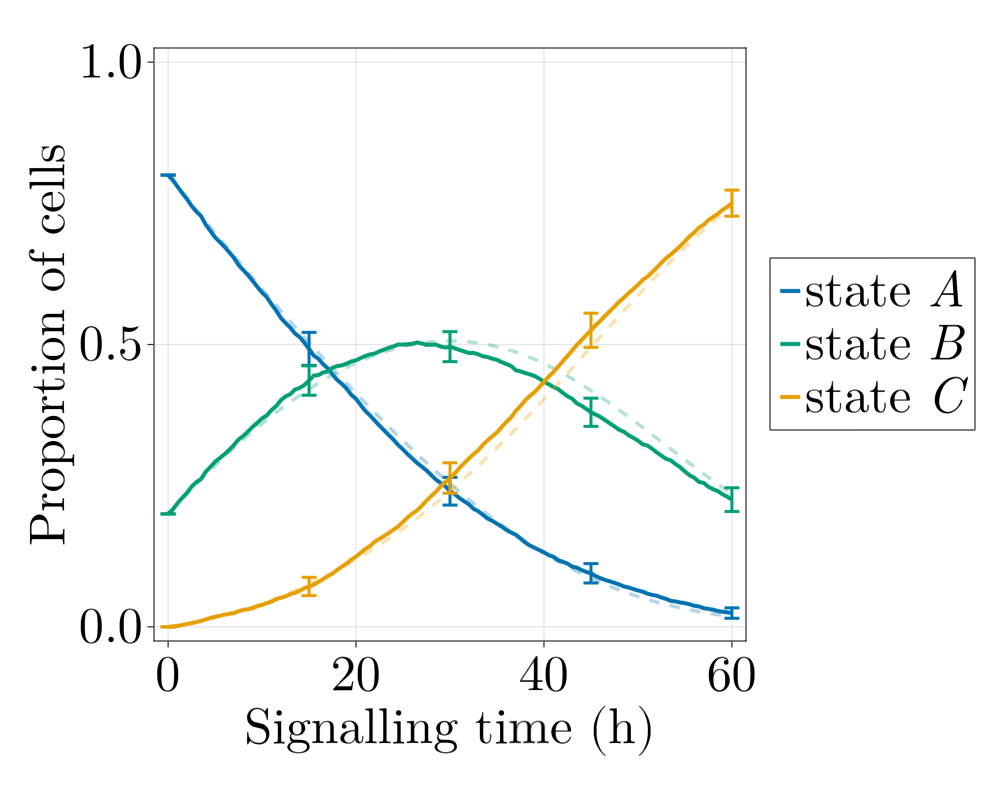
\includegraphics[width=\textwidth]{figures/405/405-proportions-simulation-cellcell-fp10-15ite.png}
        \caption{Turning on protrusions, $\rho=\rho_1$.}
    \end{subfigure}
    \caption{Proportions over time computed using the simulation. Averaged over 15 realizations. Dashed lines correspond to the mean field solution, and bars indicate the standard deviation.}
    \label{fig:prop-cellcell}
\end{figure}

Both situations showcase differences between the cell-cell signalling and the mean field approach: they begin unaltered, and at time $t=20\text{ h}$ state $B$ begins decreasing slightly faster, and state $C$ increasing slightly faster. However, cell protrusions do not seem to have an impact on cell proportions.

% Next, we compute the evolution of the proportions considering that cells proliferate to further explore the effect of protrusions. 
From now on, we focus on the cell-cell signalling case.


\subsection{Differentiation with proliferation}\label{sec:diff-prol}

The results reproduced here were obtained using Program \ref{pg:growdiff-proportions}.

In the previous experiment we disable proliferation during differentiation, gi\-ven that implementing both processes at the same time is less numerically stable. Still, this process may affect the states' evolution. We perform again the computations to ensure that, under these conditions, we can turn it off to study the aggregate. The time\-step is reduced, the initial population is $60$ and the average division time is set to $\tau_\text{div}=20\text{ h}$.

We perform a simulation using mean field feedback with proliferation and determine that, as expected, the aggregate still follows the solution. Using this as a reference, we simulate two aggregates varying the protrusion strength. The plots are shown in Figure \ref{fig:props-prolif}.

\begin{figure}[ht]
    \centering
    \begin{subfigure}{0.47\textwidth}
        \centering
        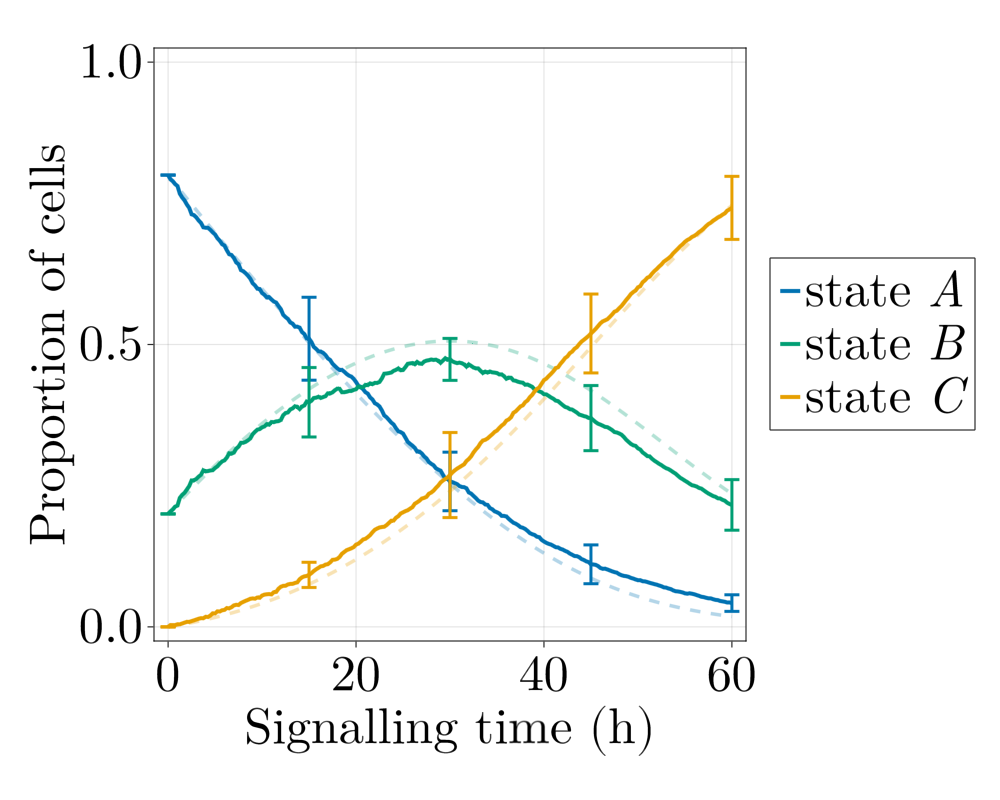
\includegraphics[width=\textwidth]{figures/406/406-proportions-diffgrow-simulation-10ite-fp0-cellcell.png}
        \caption{Cell-cell signalling, $D=0$. Averaged over 10 realizations.}
    \end{subfigure}
    \hfill
    \begin{subfigure}{0.47\textwidth}
        \centering
        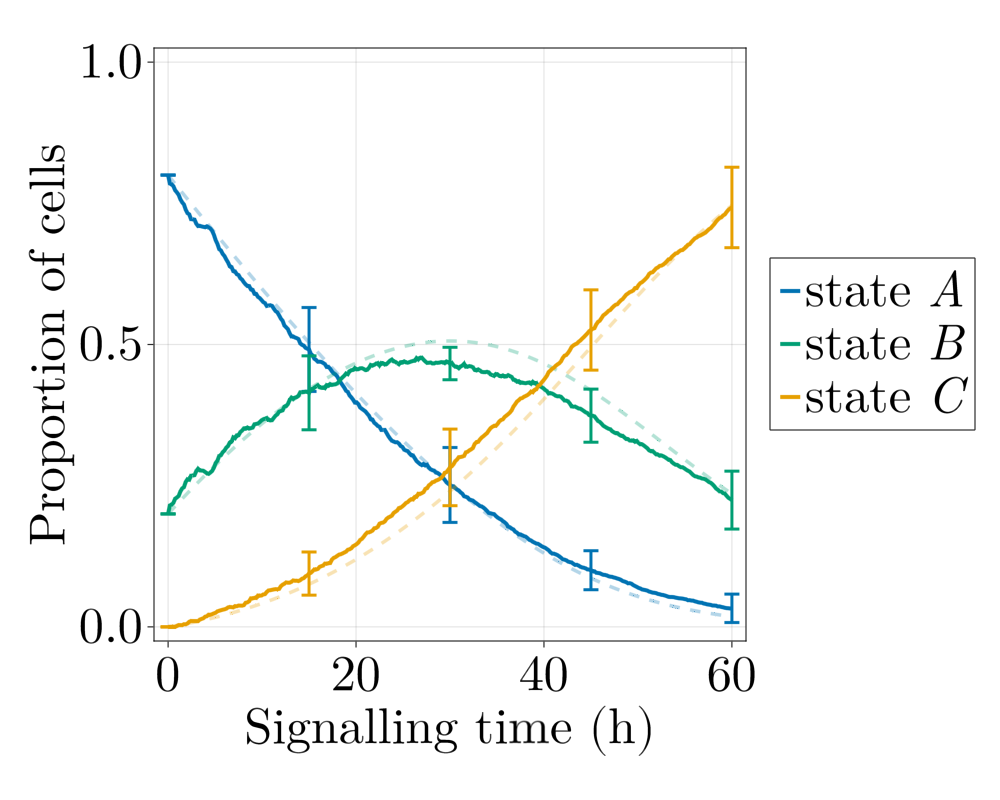
\includegraphics[width=\textwidth]{figures/406/406-proportions-diffgrow-simulation-10ite-fp10-cellcell.png}
        \caption{Cell-cell signalling, $\rho=\rho_1$. Averaged over 10 realizations.}
        \label{fig:props-prolif-rho1}
    \end{subfigure}
    % \begin{subfigure}{0.47\textwidth}
    %     \centering
    %     \includegraphics[width=\textwidth]{figures/410/410-proportions-diffgrow-simulation-10ite-fp200-cellcell-7ite.png}
    %     \caption{Cell-cell signalling, $\rho=\rho_2$. Over 7 iterations.}
    % \end{subfigure}
    % \hfill
    \begin{subfigure}{0.47\textwidth}
        \centering
        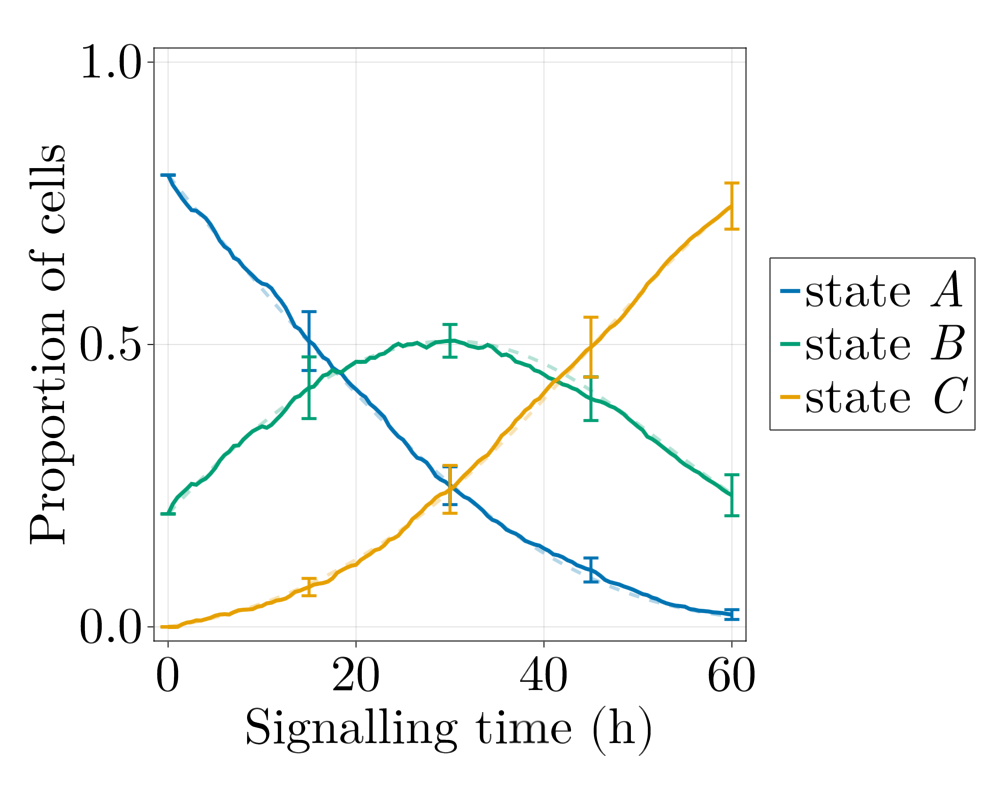
\includegraphics[width=\textwidth]{figures/406/406-proportions-diffgrow-simulation-10ite-meanfield-10ite.png}
        \caption{Mean field feedback. Averaged over 10 realizations.}
    \end{subfigure}
    \caption{Proportions over time with proliferation, compared to the mean field solution (dashed lines).}
    \label{fig:props-prolif}
\end{figure}

The stochasticity of growth makes these models very variable. Still, it seems that the states' evolution follows the same form as when cells do not proliferate. This behaviour is expected, since the rate of proliferation of all cells is the same. Using this result, we argue that, under the aforementioned conditions, we can study the differentiation process turning off differentiation.


\section[Proportion of B cells in terms of b]{Proportion of $B$ cells in terms of $b$}\label{sec:phi-b}

The results reproduced here were obtained using Program \ref{pg:phib}.

In this section, we compute the evolution of the proportion of cells in state $B$ at a fixed time $t_n$, $\phi_B(t_n)$, according to its initial proportion, $\phi_B(0)=b$. The objective of this approach is to analyse how initial cell population affects cellular differentiation and get another insight on the effect of feedback.

We will compute the function for times $t\in\{0,15,30,45,60\}$ (h). The plots for the constant and  mean field rates are shown in Figure \ref{fig:phib-solutions} to serve as a reference for the rest of the section. The analogous plots for states $A$ and $C$ in terms of $b$ are displayed in Section \ref{sec:supp} of the Appendix for the sake of completion (see Figure \ref{fig:phix-solutions}).

\begin{figure}[ht]
    \centering
    \begin{subfigure}{0.47\textwidth}
        \centering
        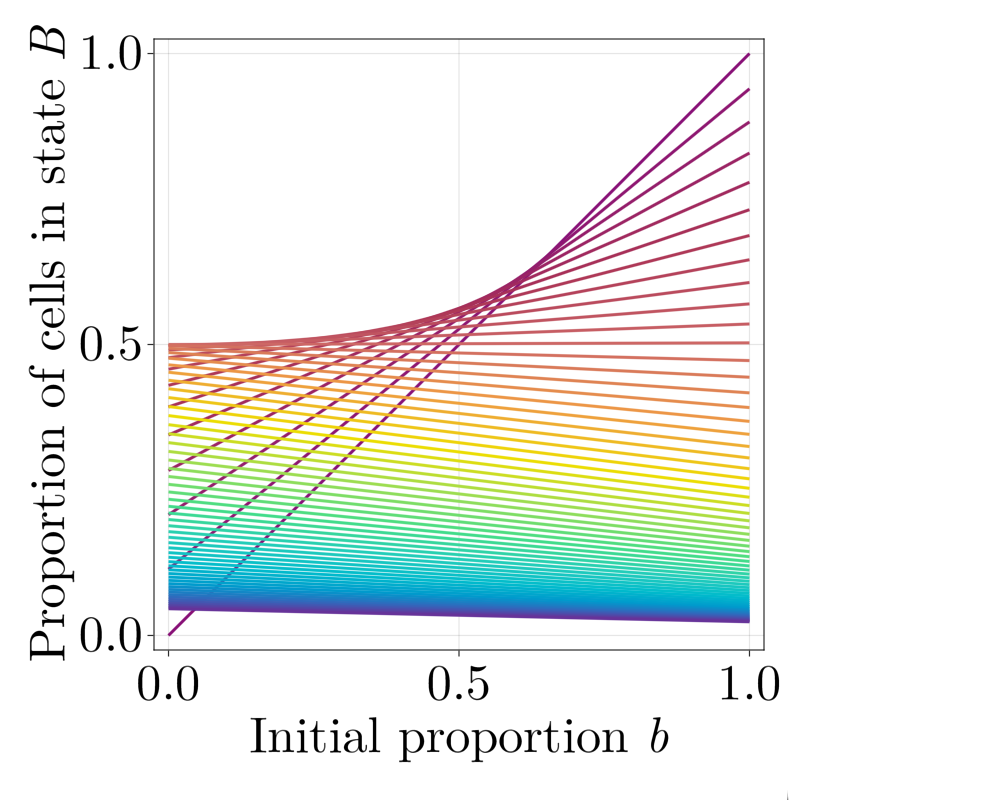
\includegraphics[width=\textwidth]{figures/407/407-phib-vs-b-solution-constant-all.png}
        \caption{Constant rates,\\time $t=0,1,...,60$ (h).}
        \label{fig:phib-solutions-1}
    \end{subfigure}
    \hfill
    \begin{subfigure}{0.47\textwidth}
        \centering
        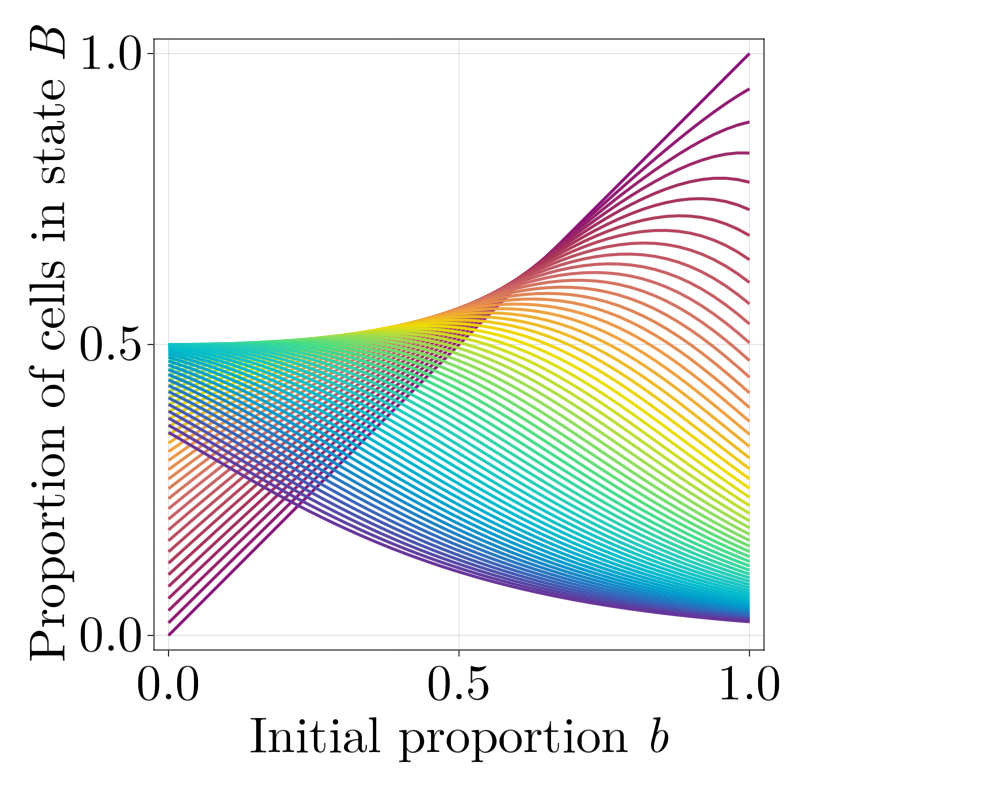
\includegraphics[width=\textwidth]{figures/407/407-phib-vs-b-solution-meanfield-all.png}
        \caption{Mean field feedback,\\time $t=0,1,...,60$ (h).}
        \label{fig:phib-solutions-2}
    \end{subfigure}
    \begin{subfigure}{0.47\textwidth}
        \centering
        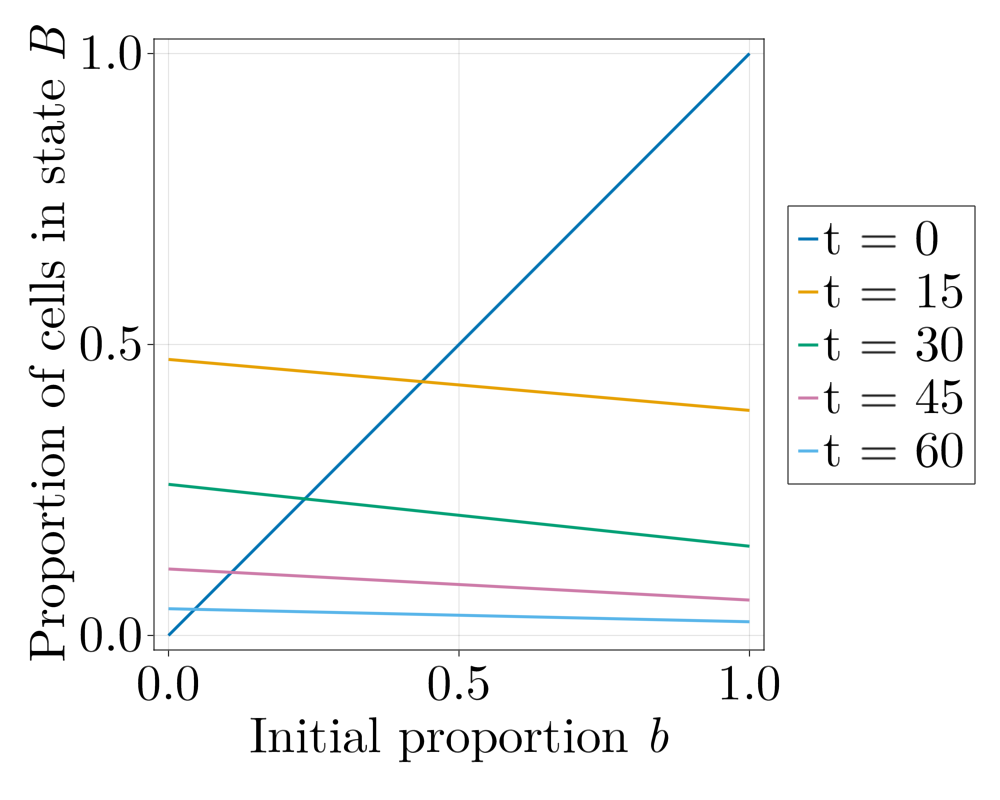
\includegraphics[width=\textwidth]{figures/407/407-phib-vs-b-solution-constant.png}
        \caption{Constant rates.}
        \label{fig:phib-solutions-3}
    \end{subfigure}
    \hfill
    \begin{subfigure}{0.47\textwidth}
        \centering
        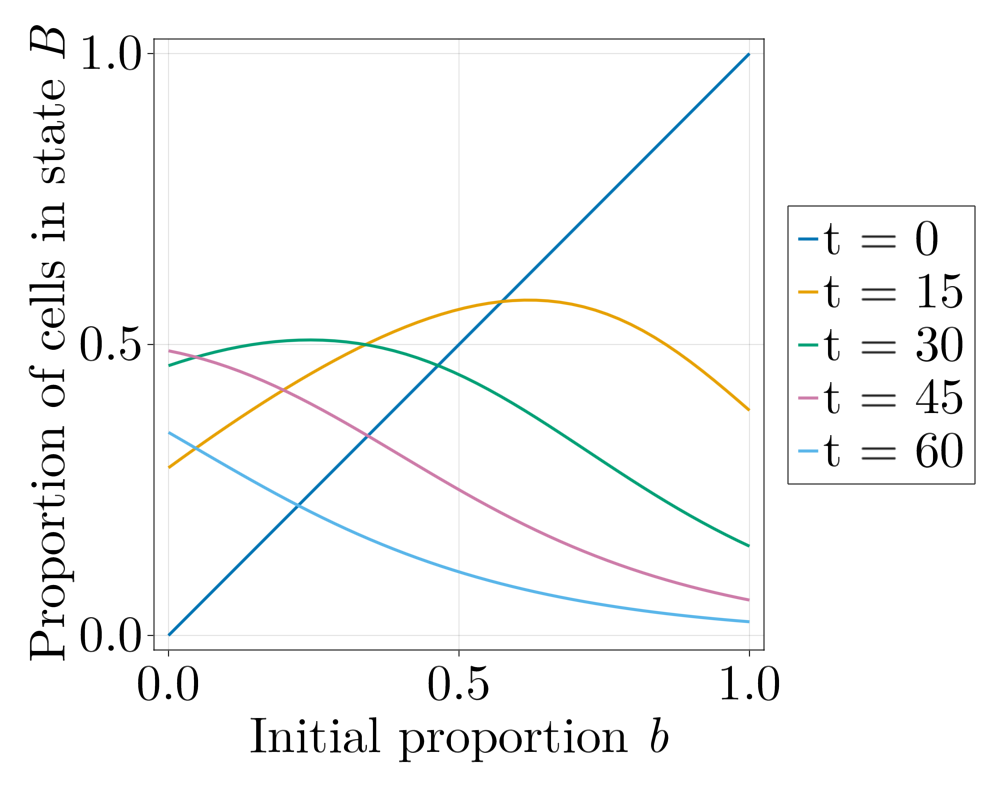
\includegraphics[width=\textwidth]{figures/407/407-phib-vs-b-solution-meanfield.png}
        \caption{Mean field feedback.}
        \label{fig:phib-solutions-4}
    \end{subfigure}
    \caption{$\phi_B(t_n)$ against $b$ using the known solutions.}
    \label{fig:phib-solutions}
\end{figure}

Let us analyse the solutions. For constant rates (or linear differentiation kinetics) the time plots rapidly  become decreasing, and in Figure \ref{fig:phib-solutions-1} the proportion of $B$ cells is always larger at $t=15\text{ h}$. This simple model can reproduce a maximum in the $B$ population (see Figure \ref{fig:prop-solutions}), still, it cannot reproduce the nonlinear dependence observed experimentally for this plot \parencite{Oriola_2025}.

For mean field feedback (a type of nonlinear differentiation kinetics), the plots for approximately the first half of the simulation exhibit a maximum, whereas the other half accomplishes its maximum proportion when $b=0$. Whenever the time plot is above than the identity line ($t=0$), the proportion of cells at that time is greater than the corresponding $b$. Unlike in the linear case, the proportion of $B$ cells increases and decreases over time, namely
\begin{align*}
    \begin{aligned}
        b &= 0: &\quad &\phi_B(45) > \phi_B(30) > \phi_B(60) > \phi_B(15) > b, \\
        b &= 0.25: &\quad &\phi_B(30) > \phi_B(15) > \phi_B(45) > b > \phi_B(60).
    \end{aligned}
\end{align*}
For small $b$, the proportion at later times is much greater than the linear case, since more cells are in state $A$ and thus inhibit the differentiation. As $b$ approaches 1, the plot resembles the linear case.

% \subsection{Equal proliferation rates}
% Consider that the proliferation rates are equal for all states when the aggregate proliferates while differentiating, as we have done until now. 

\subsection{Using cell-cell feedback}

In order to visualize the effect of feedback and protrusion force, we compute simulations using cell-cell feedback model varying $\rho$ (see Figure \ref{fig:phib-simulations}).

\begin{figure}[p]
    \centering
    \begin{subfigure}{\textwidth}
        \centering
        \begin{subfigure}{0.47\textwidth}
            \centering
            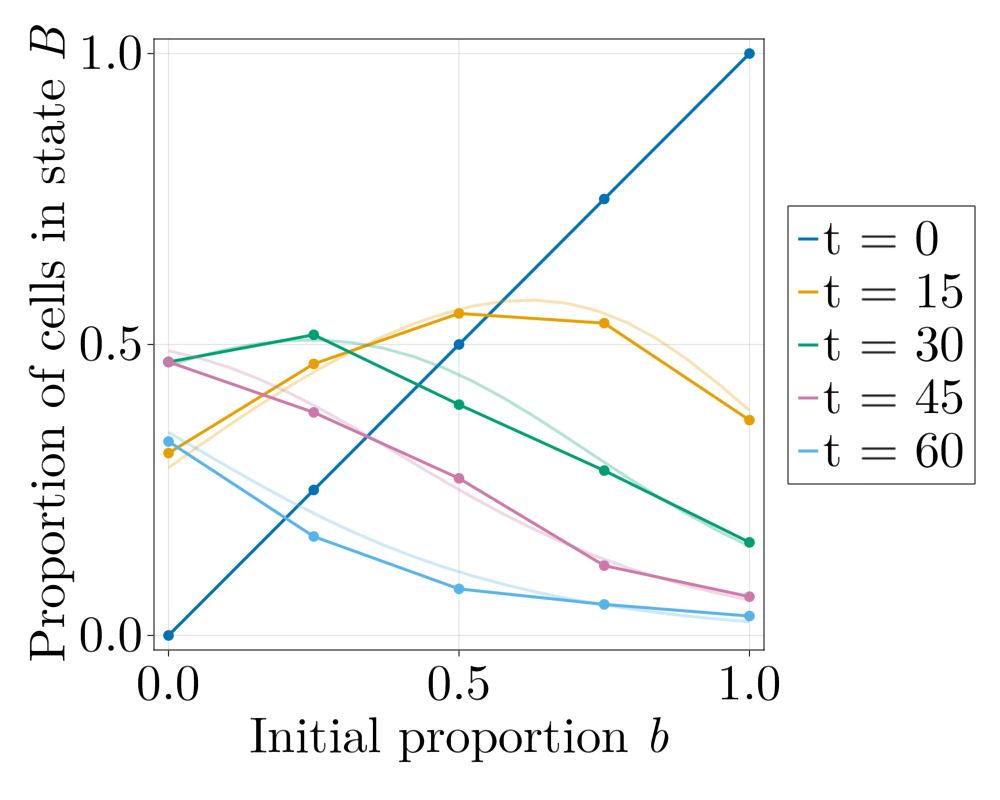
\includegraphics[width=\textwidth]{figures/407/407-phib-vs-b-simulation-1ite-fp0-vs-meanfield.png}
        \end{subfigure}
        \hfill
        \begin{subfigure}{0.47\textwidth}
            \centering
            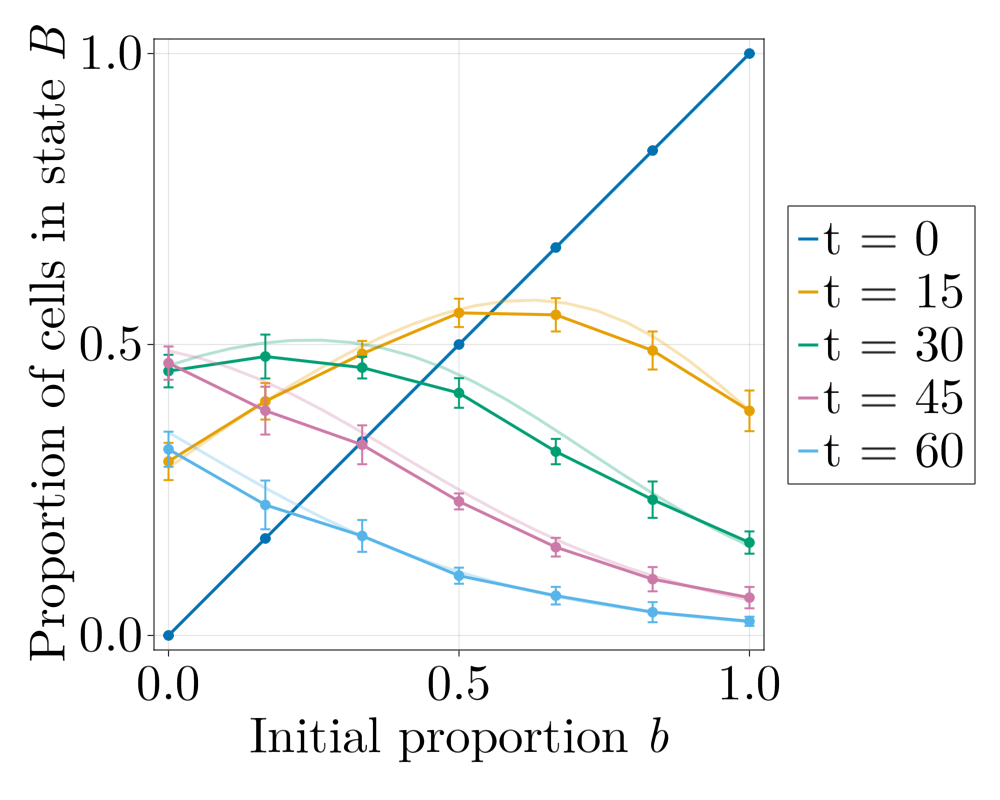
\includegraphics[width=\textwidth]{figures/408/408-phib-vs-b-simulation-10ite-fp0-cellcell-vs-meanfield.png}
        \end{subfigure}
        \caption{Using $D=0$.}
    \end{subfigure}
    \vspace{0.5em}
    \begin{subfigure}{\textwidth}
        \centering
        \begin{subfigure}{0.47\textwidth}
            \centering
            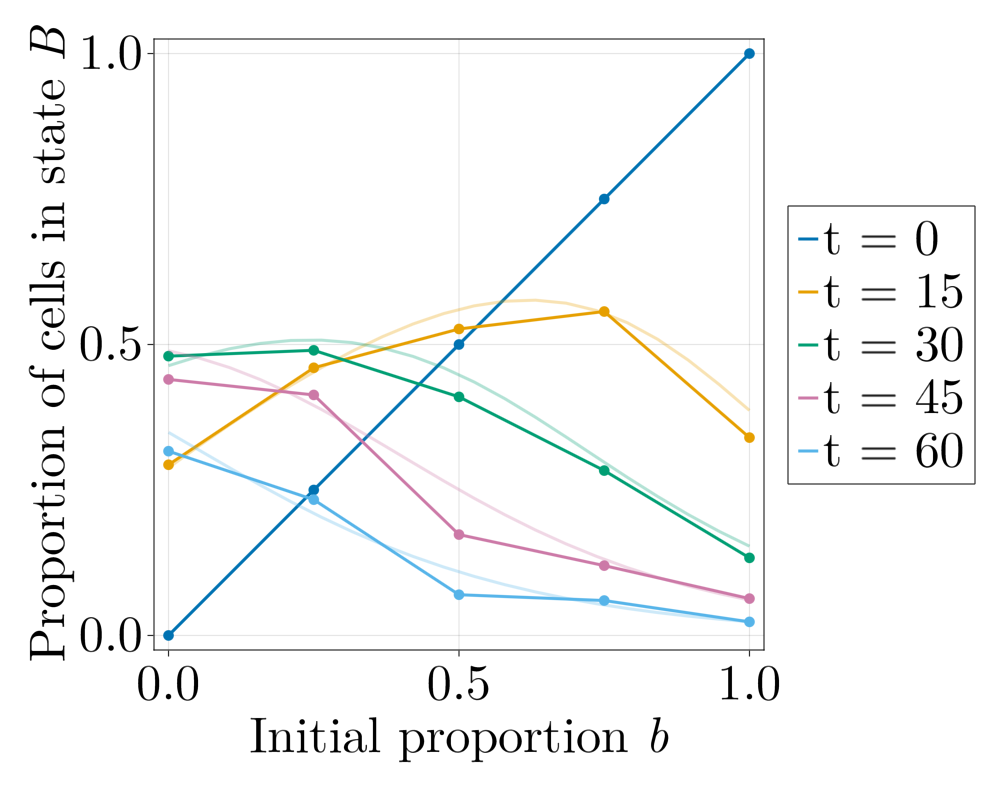
\includegraphics[width=\textwidth]{figures/407/407-phib-vs-b-simulation-1ite-fp10-vs-meanfield.png}
        \end{subfigure}
        \hfill
        \begin{subfigure}{0.47\textwidth}
            \centering
            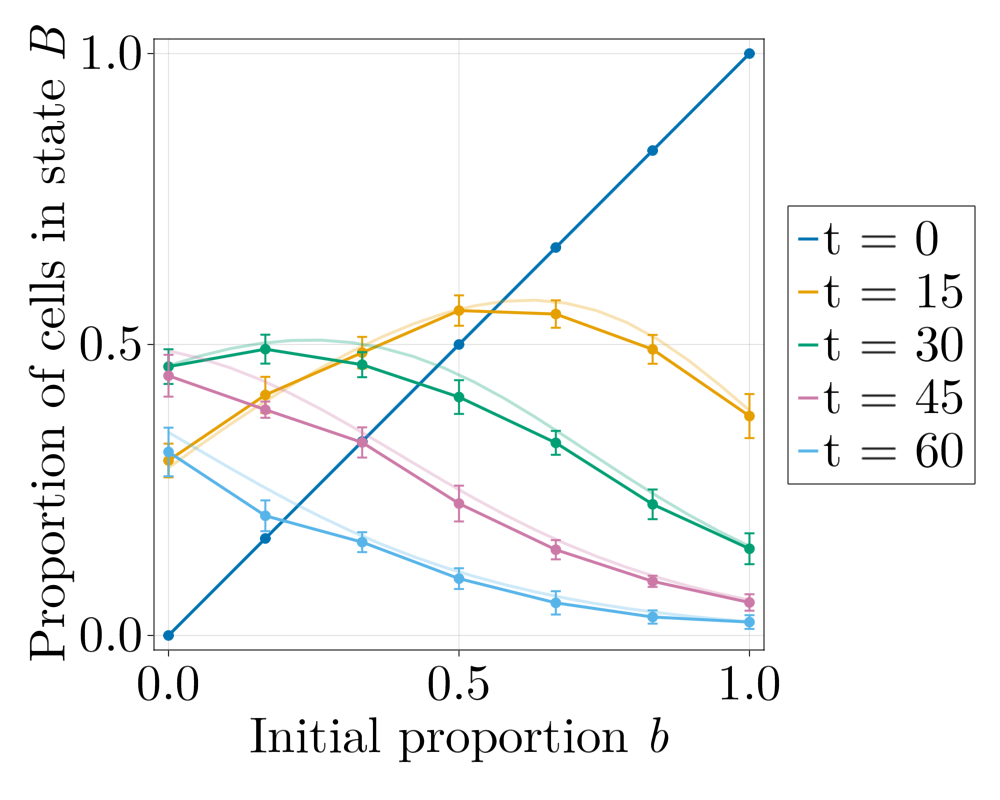
\includegraphics[width=\textwidth]{figures/408/408-phib-vs-b-simulation-10ite-fp10-cellcell-vs-meanfield.png}
        \end{subfigure}
        \caption{Using $\rho=\rho_1$.}
    \end{subfigure}
    \vspace{0.5em}
    \begin{subfigure}{\textwidth}
        \centering
        \begin{subfigure}{0.47\textwidth}
            \centering
            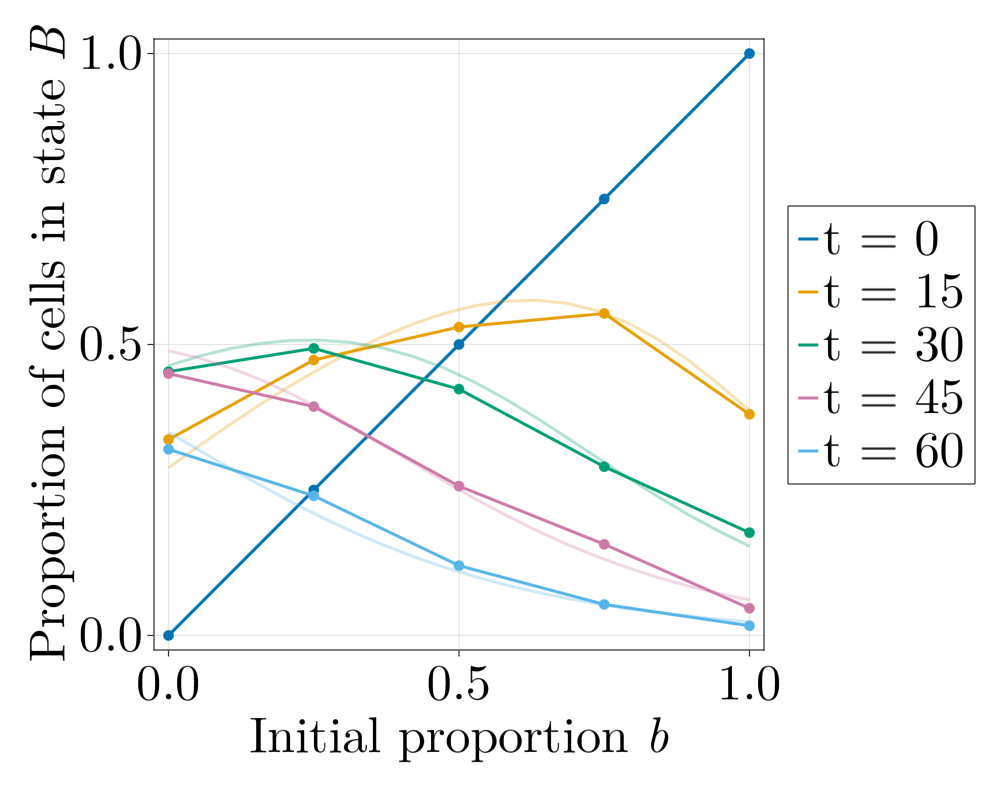
\includegraphics[width=\textwidth]{figures/407/407-phib-vs-b-simulation-1ite-fp50-vs-meanfield.png}
        \end{subfigure}
        \hfill
        \begin{subfigure}{0.47\textwidth}
            \centering
            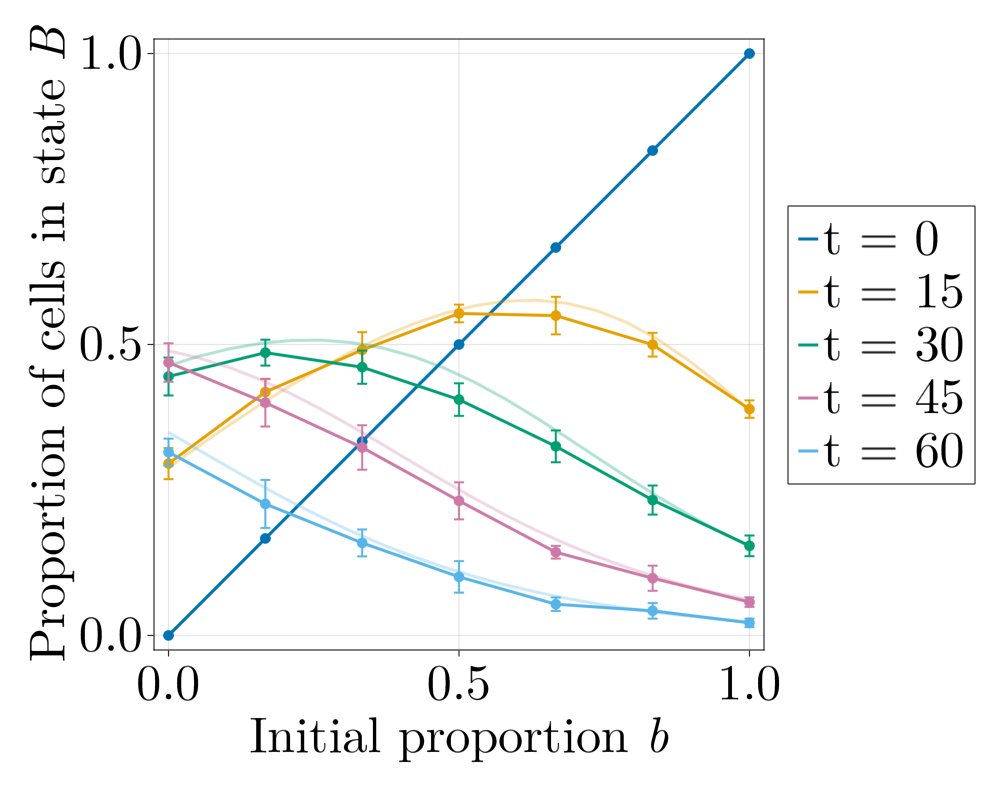
\includegraphics[width=\textwidth]{figures/408/408-phib-vs-b-simulation-10ite-fp50-cellcell-vs-meanfield.png}
        \end{subfigure}
        \caption{Using $\rho=\rho_2$.}
    \end{subfigure}
    \caption{$\phi_B(t_n)$ against $b$ using cell-cell feedback varying $\rho$, and comparing a single realization (left) to the average of 10 realizations (right). Dashed lines correspond to the mean field solution, and bars indicate the standard deviation.}
    \label{fig:phib-simulations}
\end{figure}

Obtaining one of the averages shown in Figure \ref{fig:phib-simulations} requires the simulation of 70 differentiation process, since we compute them for seven different $b$. Nevertheless, the plots to the left, which represent a realization with five $b$ points, reflect the averages. We conclude that the general behaviour of the differentiation kinetics is accurately described using this simpler method.

Regarding random cell displacements, setting $\rho=\rho_2$ does not produce visible effects with respect to $D = 0$, and $\rho=\rho_1$ displays a slightly different behaviour at some points (see $b=0$). The expected behaviour is that, for high noise, the aggregate resembles homogeneity and outputs similar results to the mean field model. However, the data obtained under the aforementioned simulation conditions does not suffice to affirm such a thing.

We further illustrate case $\rho=\rho_1$ by computing the proportion of cells in state $A$ and $C$ compared to their respective solutions (see Figure \ref{fig:phix-simulations}), so that we can observe the reason behind the changes.

\begin{figure}
    \centering
    \begin{subfigure}{0.47\textwidth}
        \centering
        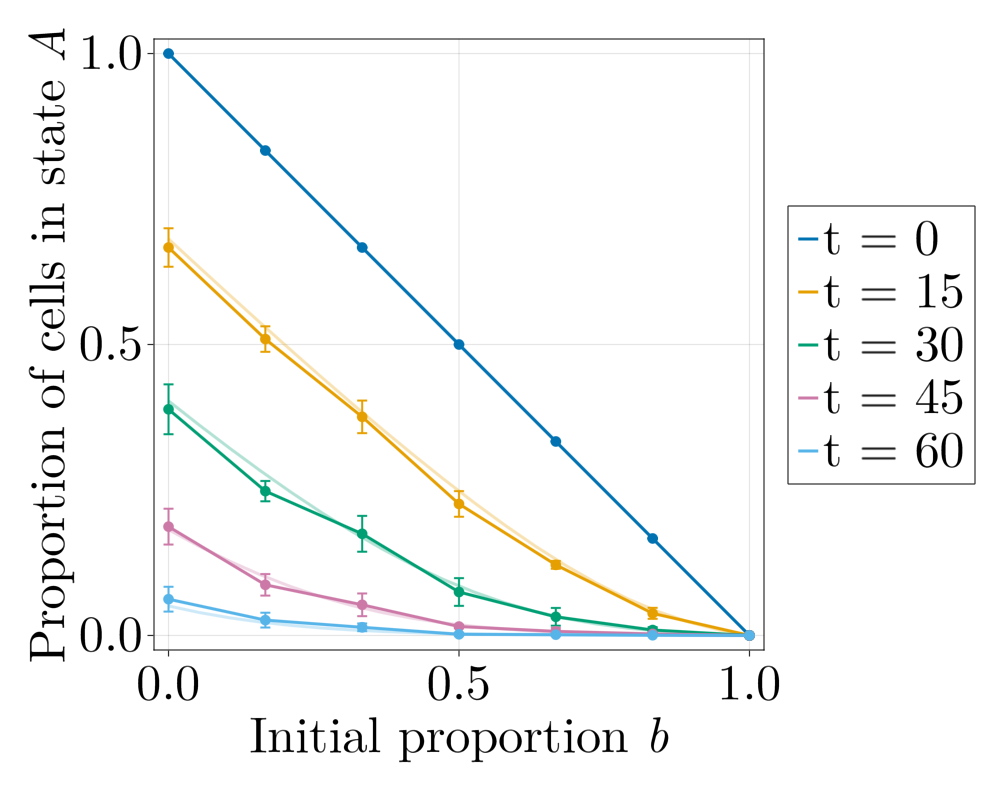
\includegraphics[width=\textwidth]{figures/408/408-phib-vs-b-simulation-10ite-fp10-cellcell-vs-meanfield-a.png}
    \end{subfigure}
    \hfill
    \begin{subfigure}{0.47\textwidth}
        \centering
        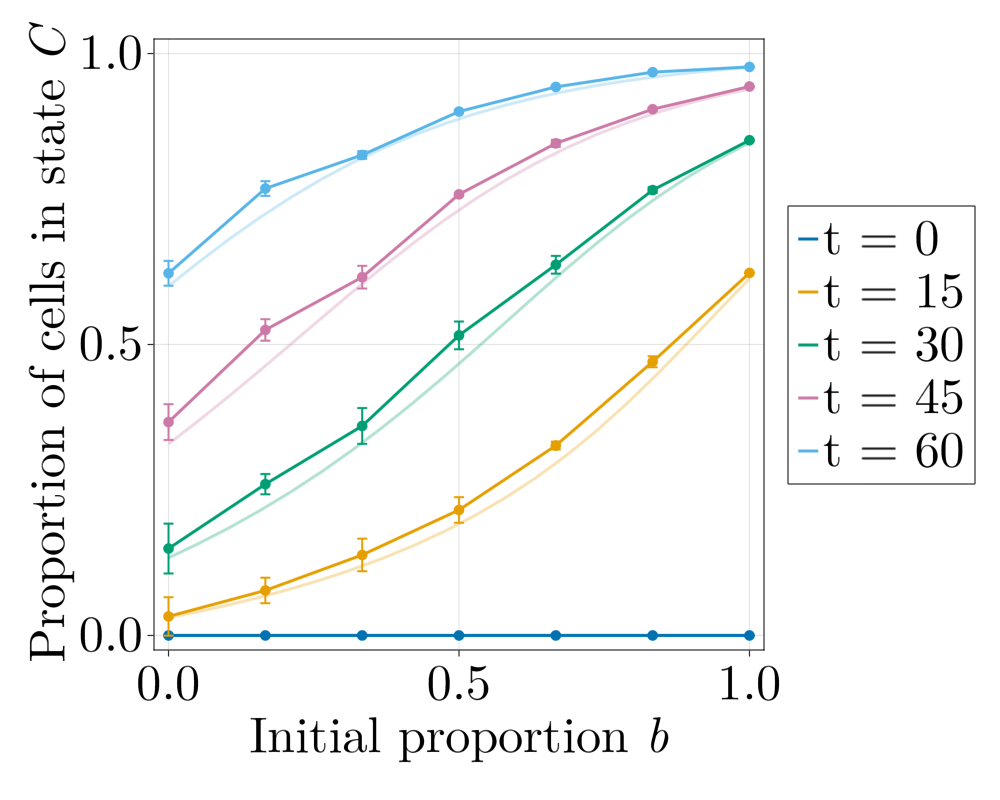
\includegraphics[width=\textwidth]{figures/408/408-phib-vs-b-simulation-10ite-fp10-cellcell-vs-meanfield-c.png}
    \end{subfigure}
    \caption{$\phi_A(t_n)$ and $\phi_C(t_n)$ against $b$ using cell-cell feedback and $\rho=\rho_1$. Averaged over 10 realizations. Dashed lines correspond to the mean field solution, and bars indicate the standard deviation.}
    \label{fig:phix-simulations}
\end{figure}


\section{Differential cell adhesion}

The results reproduced here were obtained using Programs \ref{pg:adh}, \ref{pg:adh-avgs}, and \ref{pg:adh-growing}.

In gastruloids, as cells start differentiating, cell states seem to sort and form an outer layer that surrounds the aggregate. This is thought to be a consequence of differential affinity between cells depending on their state. We visualize this process and show a succinct proportion dynamics analysis.

Working with low protrusion strength, we tune the adhesion factor so that cells in state $B$ are more attracted to each other than to the rest by a factor of $k_B$,
\begin{equation*}
    \alpha_\text{adh}(i,j)= k_B(\mathds{1}_B(i)\mathds{1}_B(j))=
    \begin{cases}
        5 &\quad \text{if $\text{state}(i)=\text{state}(j)=k_B$}\\
        0 &\quad \text{otherwise}.
    \end{cases}
\end{equation*}
We perform a parameter sweep for $k_B$ and determine to set it to 3-5 for the effect to be noticeable. A realization showing the outer layer of $C$ cells is shown in Figure \ref{fig:aggregate-layer}. We also plot the plot of $\phi_B(t_n)$ against $b$, but fail to observe any significant differences in the proportions to the previous results (see Figure \ref{fig:diff-adh-phib}).

\begin{figure}[h]
    \centering
    \begin{subfigure}{\textwidth}
        \centering
        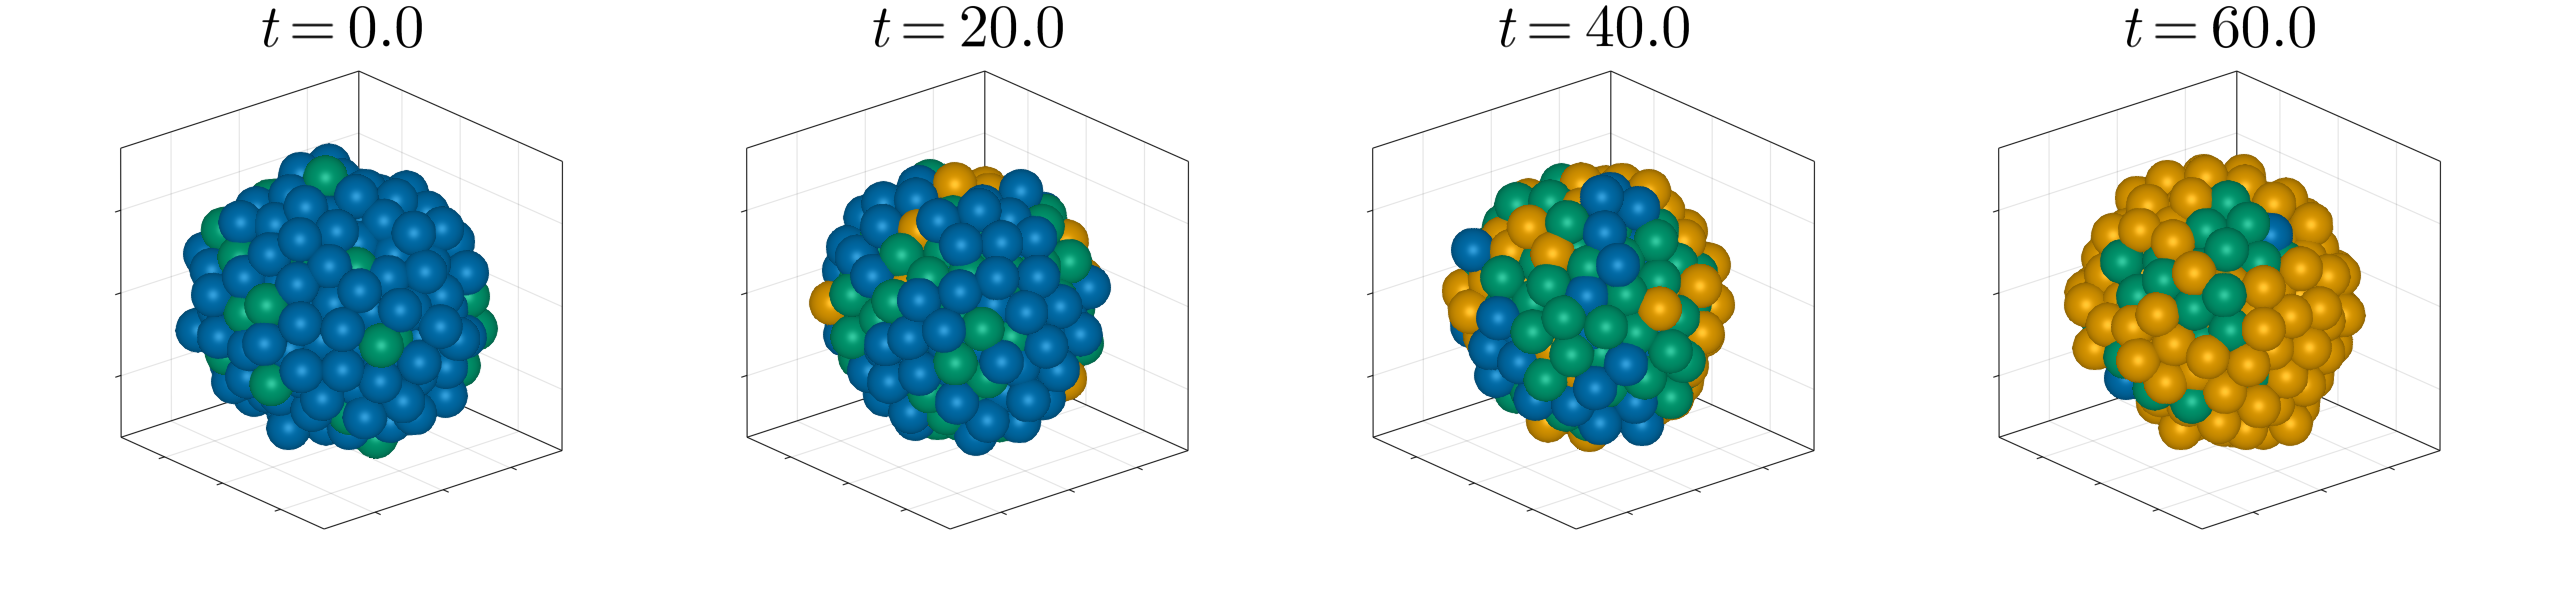
\includegraphics[width=\textwidth]{figures/409/409-aggregate-all.png}
        \caption{Visualization of all cells at each time.}
    \end{subfigure}
    \hfill
    \begin{subfigure}{\textwidth}
        \centering
        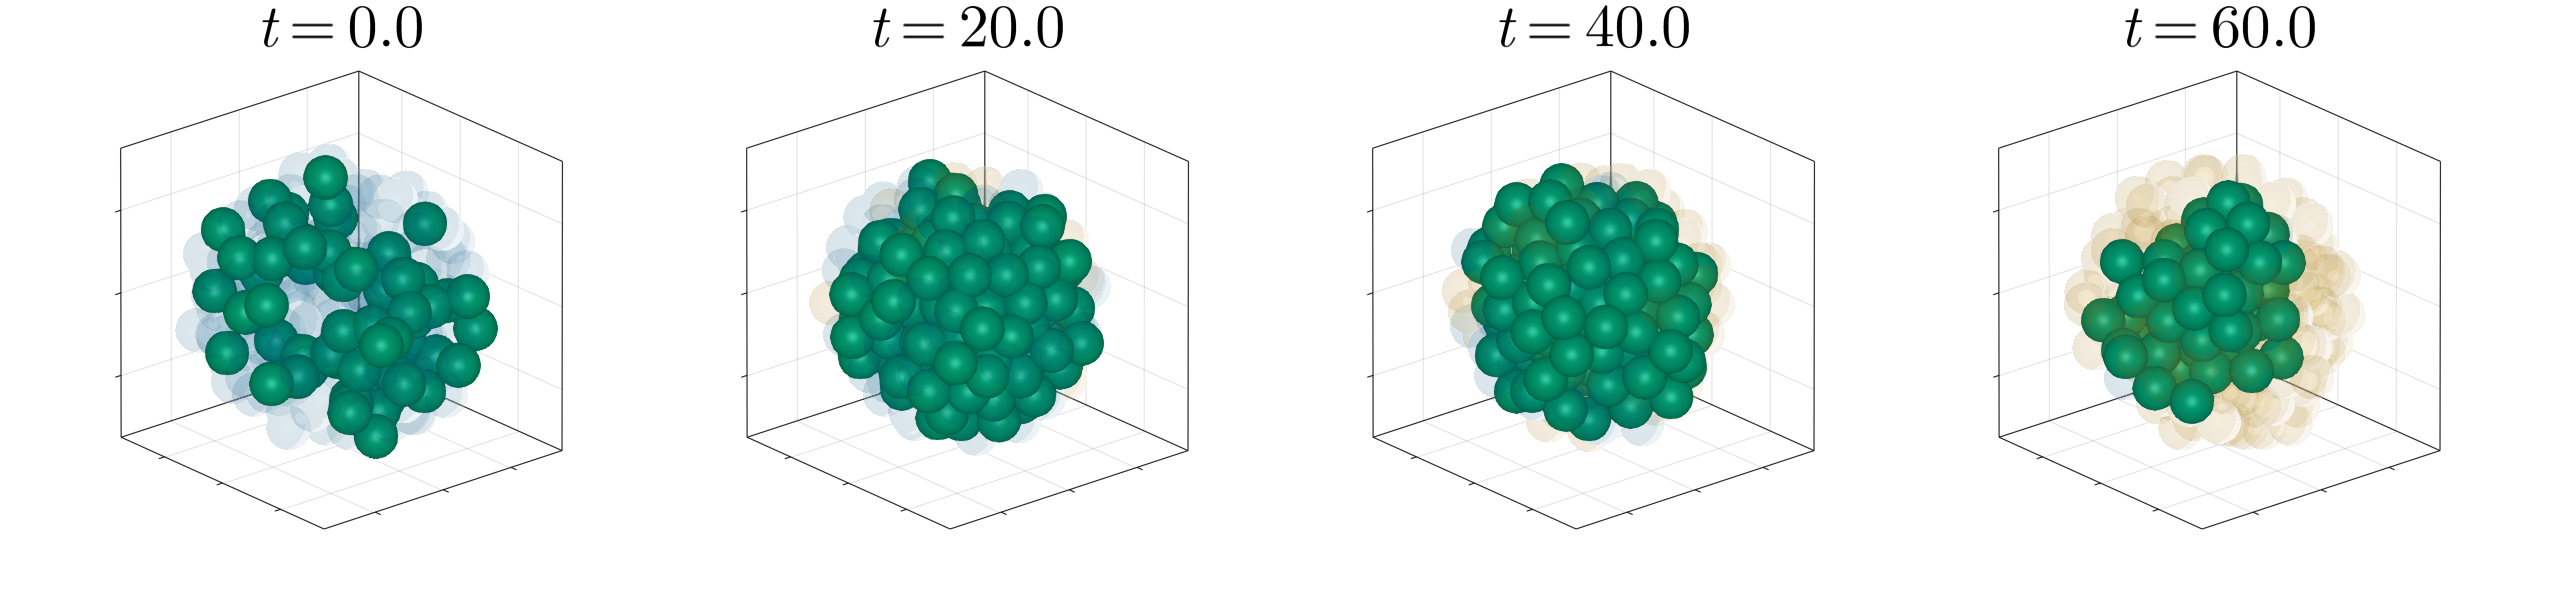
\includegraphics[width=\textwidth]{figures/409/409-aggregate-b.png}
        \caption{Visualization of the $B$ cells at each time.}
    \end{subfigure}
    \caption{Simulation of the differentiation process using differential adhesion and cell-cell feedback, for $k_B=4$. Time in hours.}
    \label{fig:aggregate-layer}
\end{figure}

\begin{figure}[h]
    \vspace{-6em}
    \centering
    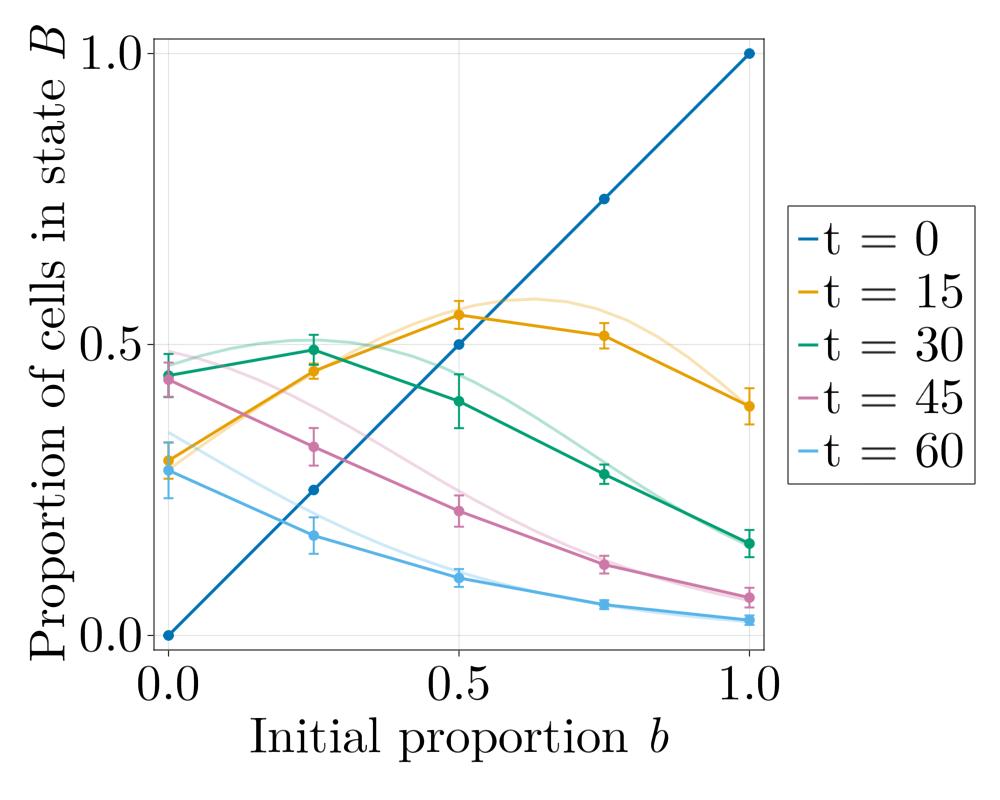
\includegraphics[width=0.47\textwidth]{figures/410/410-adhesion-phib.png}
    \caption{$\phi_B(t_n)$ against $b$ using differential adhesion, $k_B=5, \rho=\rho_1$. Averaged over 8 realizations. Dashed lines correspond to the mean field solution, and bars indicate the standard deviation.}
    \label{fig:diff-adh-phib}
\end{figure}


\subsection{Differential proliferation}

To conclude, we consider the case in which cells of a certain state have a faster average division time than the rest. The proportions over time for these cases are presented in Figure \ref{fig:diff-prolif-proportions}, computed using the same parameters for proliferating while differentiating as in Section \ref{sec:diff-prol}. The case with no proliferation (see Figure \ref{fig:diff-prolif-proportions-avg}) yields a similar result to the cell-cell signalling plots seen until now. However, the cases with proliferation evidence some differences.

In Figures \ref{fig:diff-prolif-proportions-eq} and \ref{fig:diff-prolif-proportions-b}, the proportion of $B$ cells starts larger than the mean field solution and then rapidly decreases. Figure \ref{fig:diff-prolif-proportions-a} is characterized by the high proportion of $A$ cells at the end of the differentiation. 

The differentiation process of a proliferating aggregate when $A$ cells divide faster is presented in Figure \ref{fig:diff-prolif-aggregates}.

\begin{figure}[ht]
    \centering
    \begin{subfigure}{0.47\textwidth}
        \centering
        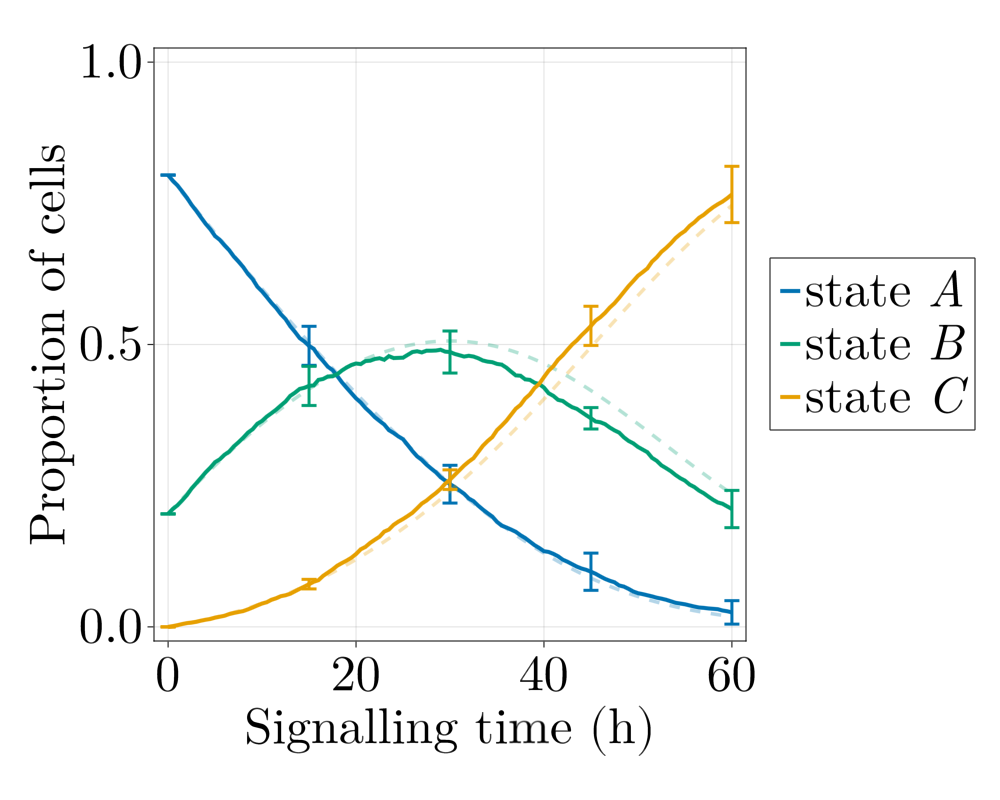
\includegraphics[width=\textwidth]{figures/410/410-adhesion-proportions-10ite-quiet.png}
        \caption{No proliferation.}
        \label{fig:diff-prolif-proportions-avg}
    \end{subfigure}
    \hfill
    \begin{subfigure}{0.47\textwidth}
        \centering
        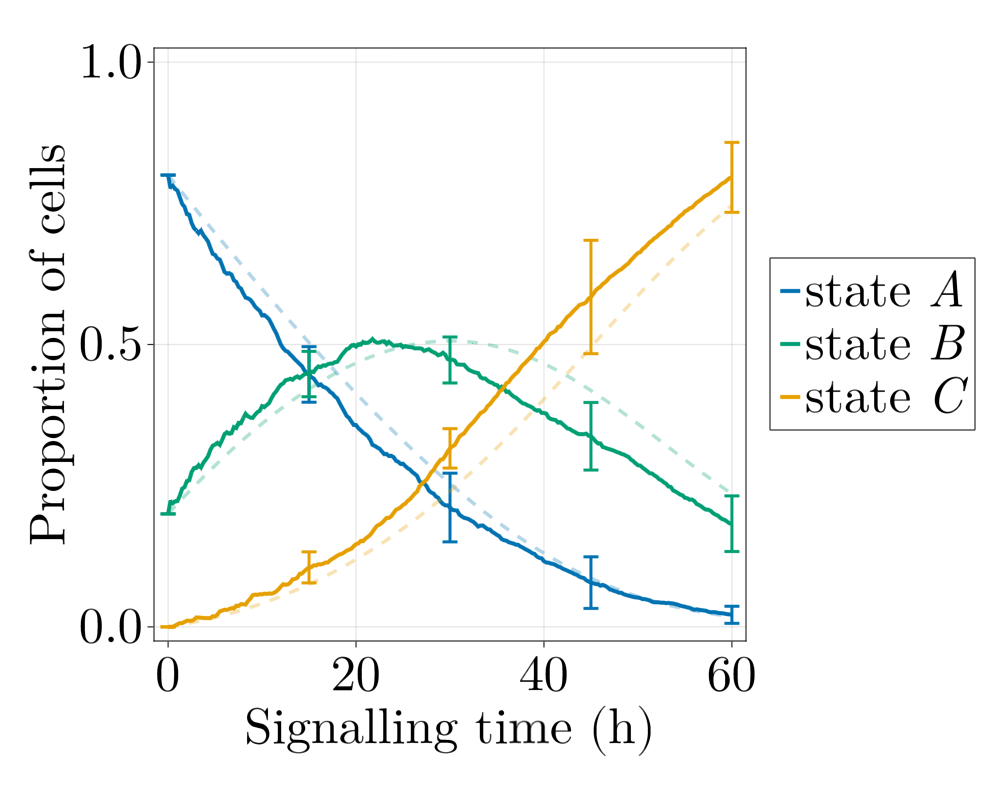
\includegraphics[width=\textwidth]{figures/411/411-adhesion-proportions-7ite-prolif-equal.png}
        \caption{Equal proliferation rates.}
        \label{fig:diff-prolif-proportions-eq}
    \end{subfigure}
    \begin{subfigure}{0.47\textwidth}
        \centering
        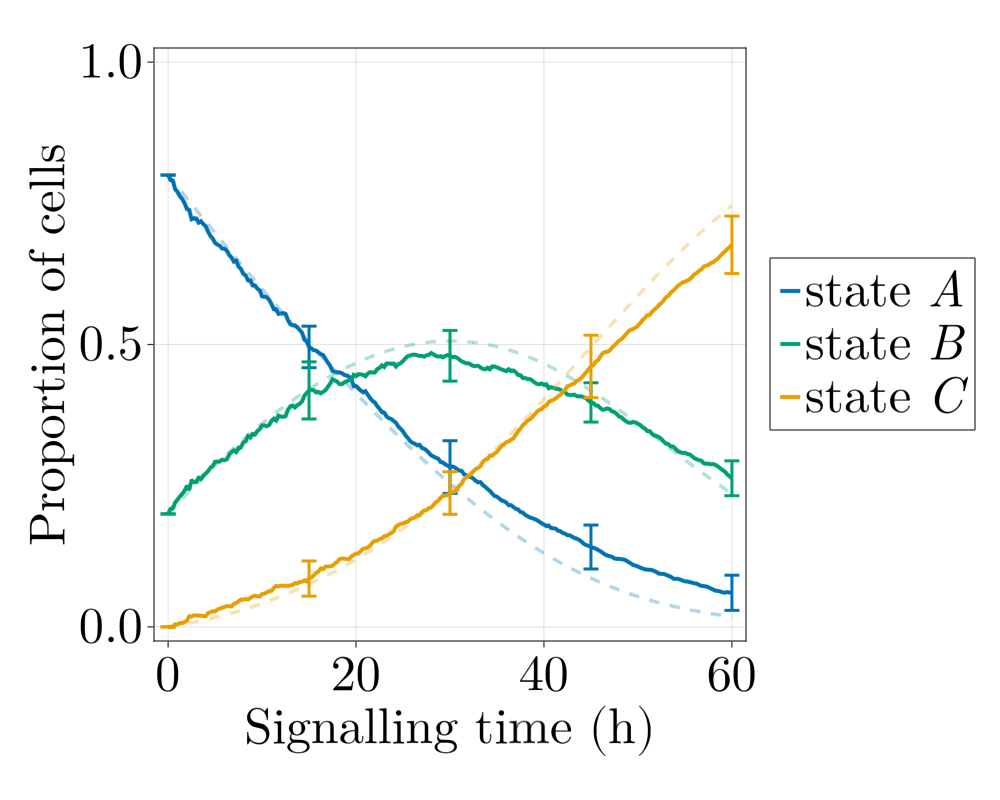
\includegraphics[width=\textwidth]{figures/411/411-adhesion-proportions-7ite-prolif-a.png}
        \caption{$A$ cells proliferate faster, $\tau_{div_A}=1.4\tau_{div_B}, \tau_{div_B}=\tau_{div_C}$.}
        \label{fig:diff-prolif-proportions-a}
    \end{subfigure}
    \hfill
    \begin{subfigure}{0.47\textwidth}
        \centering
        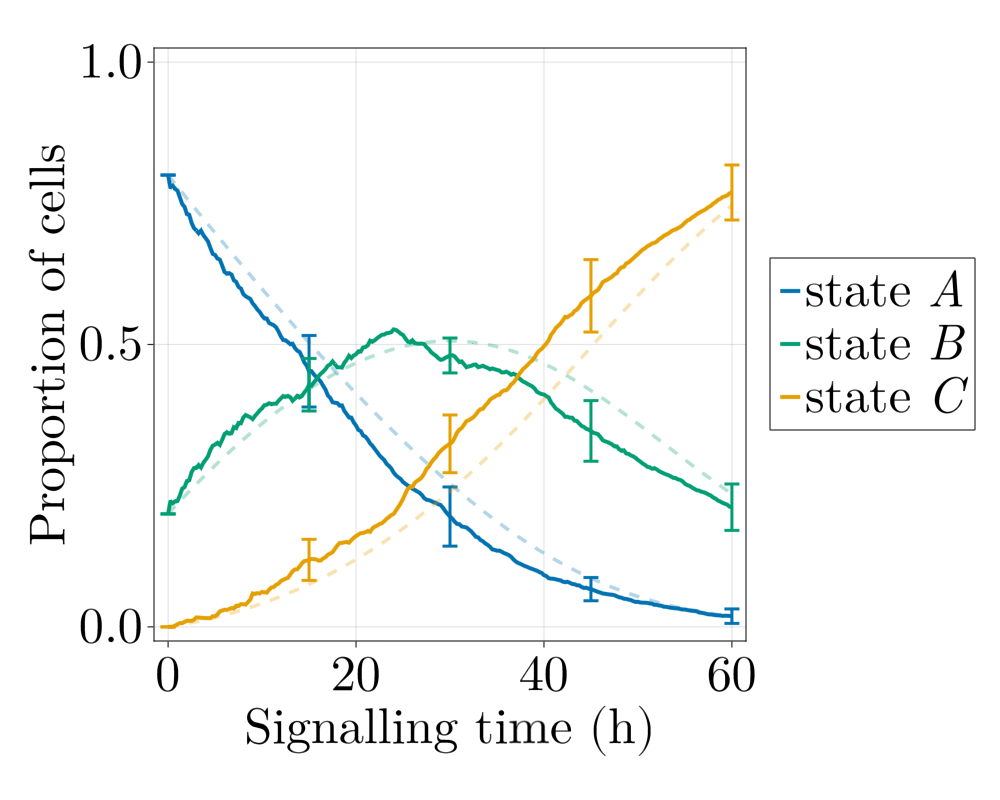
\includegraphics[width=\textwidth]{figures/411/411-adhesion-proportions-7ite-prolif-b.png}
        \caption{$B$ cells proliferate faster, $\tau_{div_B}=1.4\tau_{div_A}, \tau_{div_B}=\tau_{div_C}$.}
        \label{fig:diff-prolif-proportions-b}
    \end{subfigure}
    \caption{Proportions over time using differential adhesion and different proliferation rates, for $\tau_\text{div}=20, k_B=5, \rho=\rho_1$. Averaged over 7 realizations. Dashed lines correspond to the mean field solution, and bars indicate the standard deviation.}
    \label{fig:diff-prolif-proportions}
\end{figure}

\begin{figure}[ht]
    % \centering
    % \begin{subfigure}{\textwidth}
    %     \centering
    %     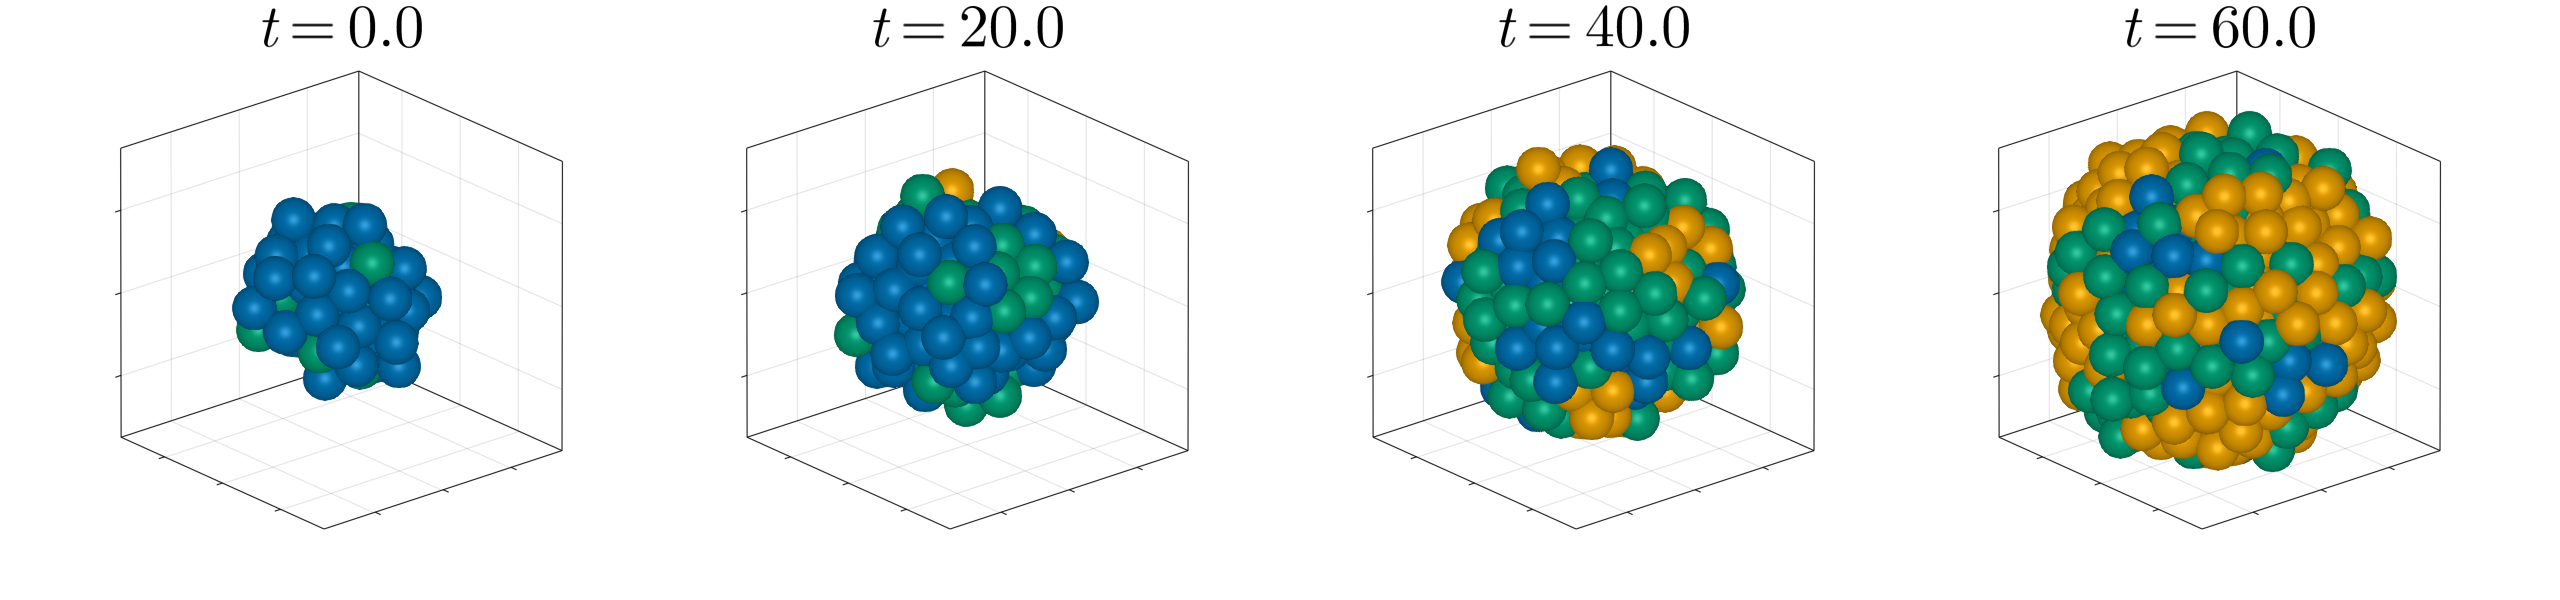
\includegraphics[width=\textwidth]{figures/411/411-aggregate-equal-all.png}
    %     \caption{Equal proliferation rates.}
    %     \label{fig:diff-prolif-proportions-eq}
    % \end{subfigure}
    % \begin{subfigure}{\textwidth}
        \centering
        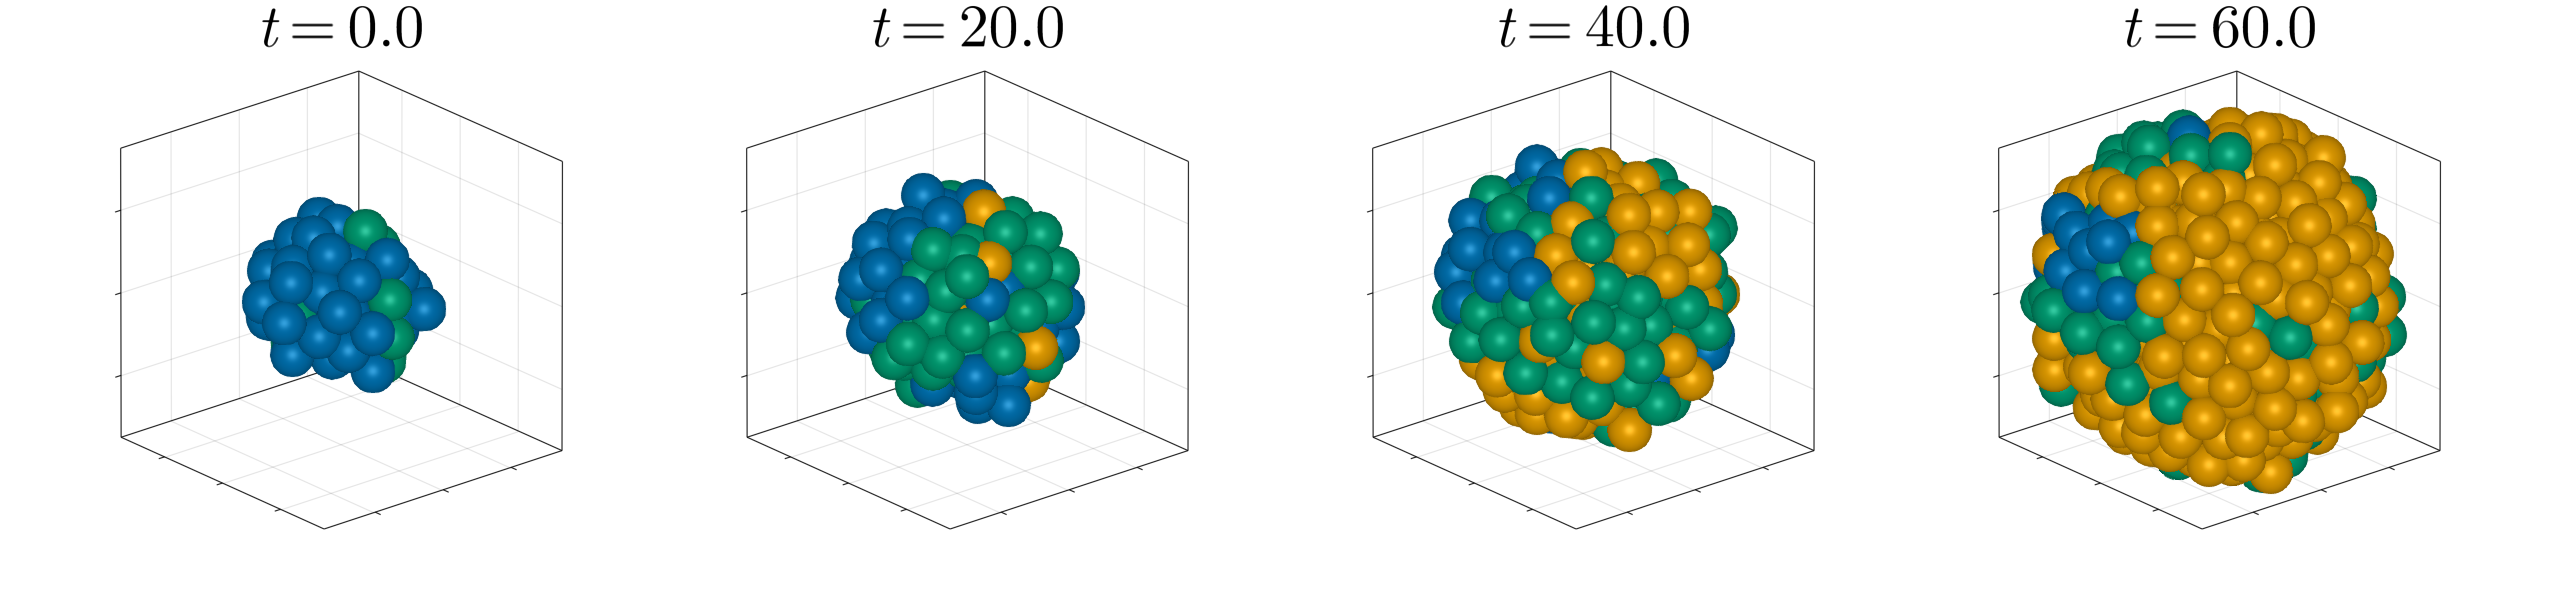
\includegraphics[width=\textwidth]{figures/411/411-aggregate-afaster-all.png}
        % \caption{$A$ cells proliferate faster, $\tau_{div_A}=1.4\tau_{div_B}, \tau_{div_B}=\tau_{div_C}$.}
        % \label{fig:diff-prolif-proportions-a}
    % \end{subfigure}
    % \hfill
    % \begin{subfigure}{\textwidth}
    %     \centering
    %     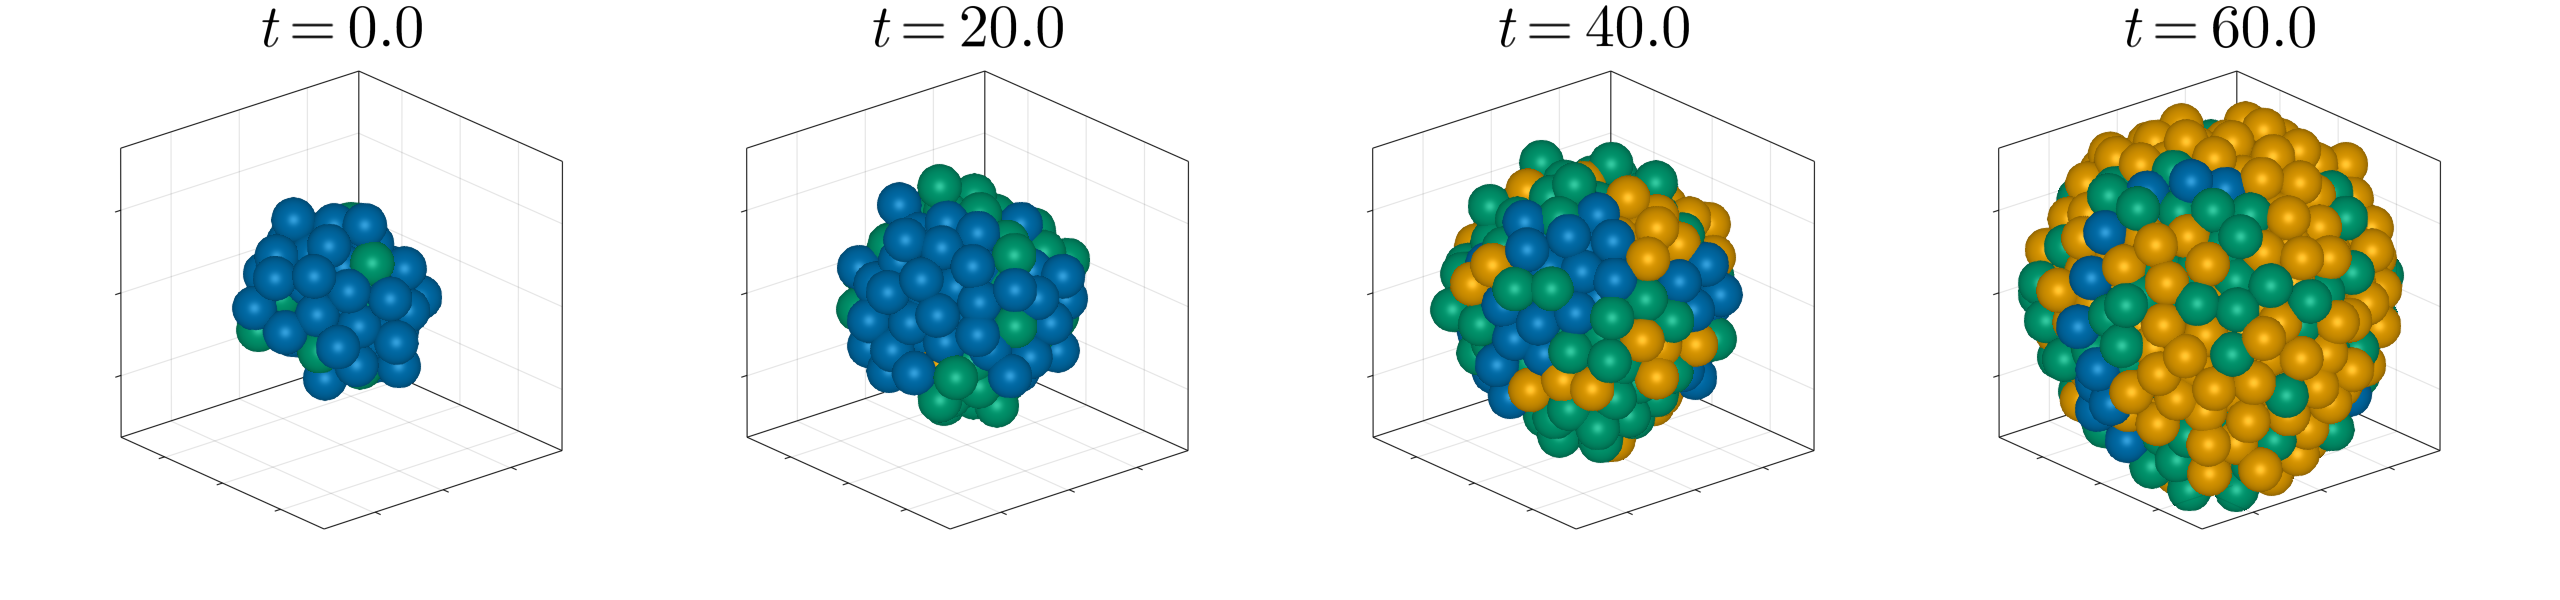
\includegraphics[width=\textwidth]{figures/411/411-aggregate-bfaster-all.png}
    %     \caption{$B$ cells proliferate faster, $\tau_{div_B}=1.4\tau_{div_A}, \tau_{div_B}=\tau_{div_C}$.}
    %     \label{fig:diff-prolif-proportions-b}
    % \end{subfigure}
    \caption{Differentiation proliferating, using differential adhesion and assuming $A$ cells proliferate faster, for $\tau_\text{div}=20, k_B=5, \rho=\rho_1$.}
    \label{fig:diff-prolif-aggregates}
\end{figure}
